% !TEX program = xelatex
% Overleaf: Menu -> Compiler -> XeLaTeX
\documentclass[12pt,a4paper]{article}
\usepackage[a4paper,margin=2.3cm]{geometry}
\usepackage{fontspec}
\setmainfont{TeX Gyre Termes}
\usepackage{babel}
\babelprovide[import,main]{vietnamese}
\usepackage{adjustbox}
\usepackage{graphicx,booktabs,float,caption,xcolor,makecell,array}
\usepackage[hidelinks]{hyperref}
\usepackage{cleveref}
\crefname{figure}{Hình}{Hình}\Crefname{figure}{Hình}{Hình}
\crefname{table}{Bảng}{Bảng}\Crefname{table}{Bảng}{Bảng}
\crefname{section}{mục}{mục}\Crefname{section}{Mục}{Mục}
\crefname{subsection}{mục}{mục}\Crefname{subsection}{Mục}{Mục}
\crefname{appendix}{phụ lục}{phụ lục}\Crefname{appendix}{Phụ lục}{Phụ lục}
\addto\captionsvietnamese{\renewcommand{\figurename}{Hình}\renewcommand{\tablename}{Bảng}%
  \renewcommand{\refname}{Tài liệu tham khảo}\renewcommand{\contentsname}{Mục lục}}
\captionsetup{font=small,labelfont=bf}
\usepackage[numbers]{natbib}
% Ô đỏ = chỗ bạn cần viết. Khi viết xong, xóa \bv{...} và dòng "% BẠN VIẾT".
\DeclareRobustCommand{\bv}[1]{\textcolor{red}{[#1]}}
\setlength{\parskip}{4pt}

\begin{document}
\begin{titlepage}
\centering
{\large \bv{Tên trường / khoa}\par}
\vspace{2.5cm}
{\LARGE\bfseries BÁO CÁO THÍ NGHIỆM\par}
\vspace{0.6cm}
{\Large CUTOFF tối ưu cho mergesort trên máy cá nhân\par}
\vspace{2.5cm}
{\large Môn: Cấu trúc dữ liệu và giải thuật\par}
\vspace{0.4cm}
{\large Sinh viên: \bv{Họ tên} \quad MSSV: \bv{MSSV} \quad Lớp: \bv{Lớp}\par}
\vspace{0.4cm}
{\large Giảng viên: \bv{Tên giảng viên}\par}
\vfill
{\large \bv{Ngày nộp}\par}
\end{titlepage}
\tableofcontents
\newpage

\section{Giới thiệu và câu hỏi nghiên cứu}\label{sec:1}
%
% - **Bối cảnh:** mergesort tốn chi phí phụ lớn với đoạn con nhỏ (lời gọi đệ quy, copy sang `aux`). Cải tiến là sắp các đoạn có độ dài ≤ CUTOFF bằng insertion sort. (BG 237)
% - **Câu hỏi thực tế:** giáo trình nêu CUTOFF = 7 (bản cũ) và 10 (bản mới) (ĐB). Vậy trên máy của tôi, giá trị nào tốt nhất?
% - **Các câu hỏi nghiên cứu:**
%   - RQ1: CUTOFF nào cho thời gian nhỏ nhất (dữ liệu ngẫu nhiên), và vùng "gần tối ưu" rộng đến đâu?
%   - RQ2: CUTOFF tối ưu thay đổi thế nào theo N và theo phân bố dữ liệu?
%   - RQ3: Mức tăng tốc tại CUTOFF = 7, 10 và tại giá trị tốt nhất so với không dùng cutoff là bao nhiêu? Có đạt "khoảng 20%" như bài giảng không? 7 hay 10 tốt hơn?
% - **Đóng góp (gạch đầu dòng ngắn):**
%   - Đo ghép cặp trên 72 giá trị N được chọn để tránh lớp tương đương. [F20]
%   - Ba lượt chạy, 9 JVM; lượt chính có typeperf xác minh xung trong suốt lượt. [F77, F78]
%   - Có số đếm phép toán đi kèm thời gian đo.
%   - Tìm và xác định cơ chế của một nguồn sai lệch hệ thống (luồng đo kẹt trên nhân 0 ở xung thấp). [mục 7.1; Phụ lục C]
%
% BẠN VIẾT:
\bv{Bạn viết nội dung phần này}


\section{Cơ sở lý thuyết}\label{sec:2}
%
% - **Mergesort top-down:** chia đôi ⌈n/2⌉ / ⌊n/2⌋, merge qua `aux`.
%   - Mệnh đề trong bài giảng: ≤ N lgN phép so sánh, ≤ 6N lgN lần truy cập mảng. (BG 233)
% - **Insertion sort:**
%   - Ngẫu nhiên: ~¼N² so sánh và ~¼N² đổi chỗ.
%   - Đã sắp: N − 1 so sánh, 0 đổi chỗ.
%   - Đảo ngược: ~½N² so sánh và ~½N² đổi chỗ. (BG 205, 207)
%   - Hệ quả cho phần thảo luận: chi phí trên một lá độ dài k phụ thuộc mạnh vào thứ tự dữ liệu trong lá.
% - **Vì sao cutoff có thể giúp** (nêu dạng giả thuyết, phần 6 sẽ kiểm chứng):
%   - Bỏ khoảng lg(độ dài lá) tầng merge ở đáy cây.
%   - Bỏ lời gọi đệ quy cho đoạn nhỏ.
%   - Insertion sort làm việc trên vùng nhớ liền kề, nhỏ, không phải copy sang `aux`.
% - **Đánh đổi:** insertion sort có chi phí bậc hai theo độ dài lá, nên tồn tại một độ dài lá tối ưu.
% - **Nhận định của bài giảng:** "Thêm một dòng... có thể nhanh hơn khoảng 20%". (BG 237)
%   - Ghi rõ hai cách đọc: thời gian giảm 20% (r = 0.80), hoặc nhanh hơn 1.2 lần (r ≈ 0.833).
% - **Định nghĩa dùng trong báo cáo:**
%   - Đoạn có độ dài ≤ CUTOFF được sắp bằng insertion sort.
%   - CUTOFF = 1 là baseline.
%   - r = T(c)/T(1); thời gian giảm = 1 − r; tăng tốc = 1/r.
%
% BẠN VIẾT:
\bv{Bạn viết nội dung phần này}


\section{Cài đặt và kiểm thử tính đúng}\label{sec:3}
%
% - **Cài đặt** (bạn tự viết từ BG buổi 4–5):
%   - Top-down; `aux` cấp phát một lần; CUTOFF là tham số.
%   - Tắt các cải tiến "dừng nếu a[mid] ≤ a[mid+1]" và "tráo vai trò mảng phụ".
%   - Chặn `cutoff < 1`.
% - **Tính ổn định (stable):**
%   - Trong merge, `less(aux[j], aux[i])` là so sánh chặt nên khi bằng khóa sẽ lấy nửa trái trước.
%   - Insertion sort chỉ đổi chỗ khi nhỏ hơn chặt.
% - **Bản đếm `MergeCutoffCounted`:**
%   - Chép từ `MergeCutoff`, bỏ `assert`, chèn bộ đếm C, A, E, S.
%   - Quy ước Sedgewick: `exch` = 4 truy cập; copy sang `aux` = 2 truy cập mỗi phần tử.
%   - Bản này không dùng để đo thời gian.
% - **Bảng 1. Các nhóm kiểm thử** (`results/correctness_test_output.txt`; tổng [F01]):
%   - Liệt kê 15 nhóm 00–14 kèm số lần kiểm tra.
%   - Nêu các kiểm tra độc lập:
%     - S bằng kết quả mô phỏng cây đệ quy.
%     - E bằng số nghịch thế trên các lá.
%     - Bản đo (`MergeCutoff`) có cùng cây đệ quy với bản đếm, kiểm tra qua số `compareTo`.
% - **Bảng 2. Mutation test** [F02] (nguồn: LOG, chạy trên sandbox JDK 21):
%   - 4 bản cài lỗi, bản nào cũng bị phát hiện.
%   - Lỗi "lệch 1 ở dòng cutoff" chỉ bị nhóm 14 bắt được. Đây là lý do cần nhóm 14.
%   - ⚠ Nếu muốn ghi mutation test là kết quả của mình, nên chạy lại trên máy bạn.
% - **Chú thích gợi ý:** "Bảng 1. Các nhóm kiểm thử tính đúng; tổng 970 425 lần kiểm tra, 0 lỗi (JDK 25, `-ea`)."
%
% BẠN VIẾT:
\bv{Bạn viết nội dung phần này}

\begin{table}[H]
\centering
% Gợi ý chú thích (từ dàn ý): Các nhóm kiểm thử tính đúng; tổng 970 425 lần kiểm tra, 0 lỗi (JDK 25, -ea).
\caption{\bv{viết chú thích}}
\label{tab:correctness}
\small
\begin{adjustbox}{max width=\linewidth}% Bảng: các nhóm của CorrectnessTest (results/correctness_test_output.txt)
% Sinh tự động bởi report/make_tables.py, KHÔNG sửa tay.
\begin{tabular}{rp{0.62\linewidth}rr}
\toprule
Nhóm & Nội dung kiểm tra & PASS & FAIL \\
\midrule
00 & JVM runs with -ea & 1 & 0 \\
01 & DataGenerator: values, encoding, determinism, plan & 266 & 0 \\
02 & isSorted (N=0..300 $\times$ cutoff=1..70 $\times$ 5 distributions) & 105\,350 & 0 \\
03 & output is a permutation of input (vs Arrays.sort) & 105\,350 & 0 \\
04 & MergeCutoff $=$ MergeCutoffCounted (same objects, same order) & 105\,350 & 0 \\
05 & stability (Item(key, idx)) & 126\,420 & 0 \\
06 & cutoff < 1 $\to$ IllegalArgumentException & 32 & 0 \\
07 & 1/2 N lgN $\le$ C $\le$ N lgN (cutoff=1, N=2\^{}k) & 85 & 0 \\
08 & S = N(lgN - m) (N=2\^{}k, cutoff=2\^{}m, m<k) & 403 & 0 \\
09 & S = simulated recursion tree (independent) & 105\,350 & 0 \\
10 & A = 4S + 2C + 4E & 105\,668 & 0 \\
11 & E = inversions of original array on leaves (independent) & 105\,350 & 0 \\
12 & insertion alone: sorted / reversed, k=1..50 & 100 & 0 \\
13 & no unexpected exception & 105\,350 & 0 \\
14 & MergeCutoff (timed version) has same tree: compares match & 105\,350 & 0 \\
\midrule
 & Tổng & 970\,425 & 0 \\
\bottomrule
\end{tabular}
\end{adjustbox}
\end{table}

\begin{table}[H]
\centering
% Gợi ý chú thích (từ dàn ý): Mutation test: 4 bản cài lỗi, bản nào cũng bị phát hiện (chạy trên sandbox của AI, JDK 21).
\caption{\bv{viết chú thích}}
\label{tab:mutation}
\small
\begin{adjustbox}{max width=\linewidth}% Bảng: mutation test (4 bản lỗi; chạy trên sandbox của AI, JDK 21; nguồn: log AI)
% Sinh tự động bởi report/make_tables.py, KHÔNG sửa tay.
\begin{tabular}{p{0.55\linewidth}l}
\toprule
Bản cài lỗi cố ý & Nhóm kiểm thử báo FAIL \\
\midrule
merge lấy nửa phải khi hai khóa bằng nhau & 04, 05, 14 \\
dòng cutoff lệch 1: \texttt{hi <= lo + cutoff} & chỉ 14 \\
insertion sort: \texttt{j > lo + 1} & 02, 03, 04, 05, 13, 14 \\
\texttt{mid = lo + (hi - lo + 1)/2} & 13 (StackOverflow), 14 \\
\bottomrule
\end{tabular}
\end{adjustbox}
\end{table}


\section{Thiết kế thí nghiệm}\label{sec:4}
%
% BẠN VIẾT:
\bv{Bạn viết nội dung phần này}


\subsection{Dữ liệu}\label{sec:4-1}
% (dàn ý) [F03–F06]
%   - 5 phân bố:
%     - random: hoán vị của OFFSET..OFFSET+N−1.
%     - sorted.
%     - reversed.
%     - nearly sorted: ⌊N/100⌋ lần đổi chỗ.
%     - few distinct: 10 giá trị.
%   - Mọi giá trị ≥ 1 000 000 nên không đối tượng nào dùng Integer cache.
%   - Seed cố định: `10^7·distId + N`. Định dạng nhị phân int32 kèm `manifest.csv` có sha256; chế độ `--verify`.
%   - Kiểm tra chéo: sha256 của manifest và của counts.csv trùng nhau giữa sandbox và máy bạn. [F05, F06]
% BẠN VIẾT:
\bv{Bạn viết nội dung phần này}


\subsection{Vì sao không dùng N = $2^{k}$: lớp tương đương}\label{sec:4-2}
% (dàn ý) [F18–F20]
%   - Với N = 2^k, mọi CUTOFF trong [2^m, 2^(m+1) − 1] cho cùng một cây đệ quy.
%   - Lưới 35 CUTOFF vì vậy chỉ cho 7 cây khác nhau: [1], [2–3], [4–7], [8–15], [16–31], [32–48], [64].
%   - Hệ quả: CUTOFF = 7 và 10 ứng với "lá 4" và "lá 8"; các CUTOFF trong cùng lớp chỉ khác nhau do nhiễu.
%   - Thiết kế chọn: 24 N hình học mỗi thang, N_j = round(S·2^(j/24)), S ∈ {2^12, 2^16, 2^19}.
%     - Mỗi c trong 2..32 đổi cây ở ít nhất 2 N.
%     - Tập con 8 N (thiết kế ban đầu) có 17 giá trị c đổi cây ở dưới 2 N. (T:tree_coverage)
%   - **Hình gợi ý: F:fig05.** "Hình 5. Ở N = 2^k, các CUTOFF trong cùng một dải cho cùng cây đệ quy (cùng S); chênh lệch r bên trong một dải là nhiễu đo."
% BẠN VIẾT:
\bv{Bạn viết nội dung phần này}

\begin{figure}[H]
\centering
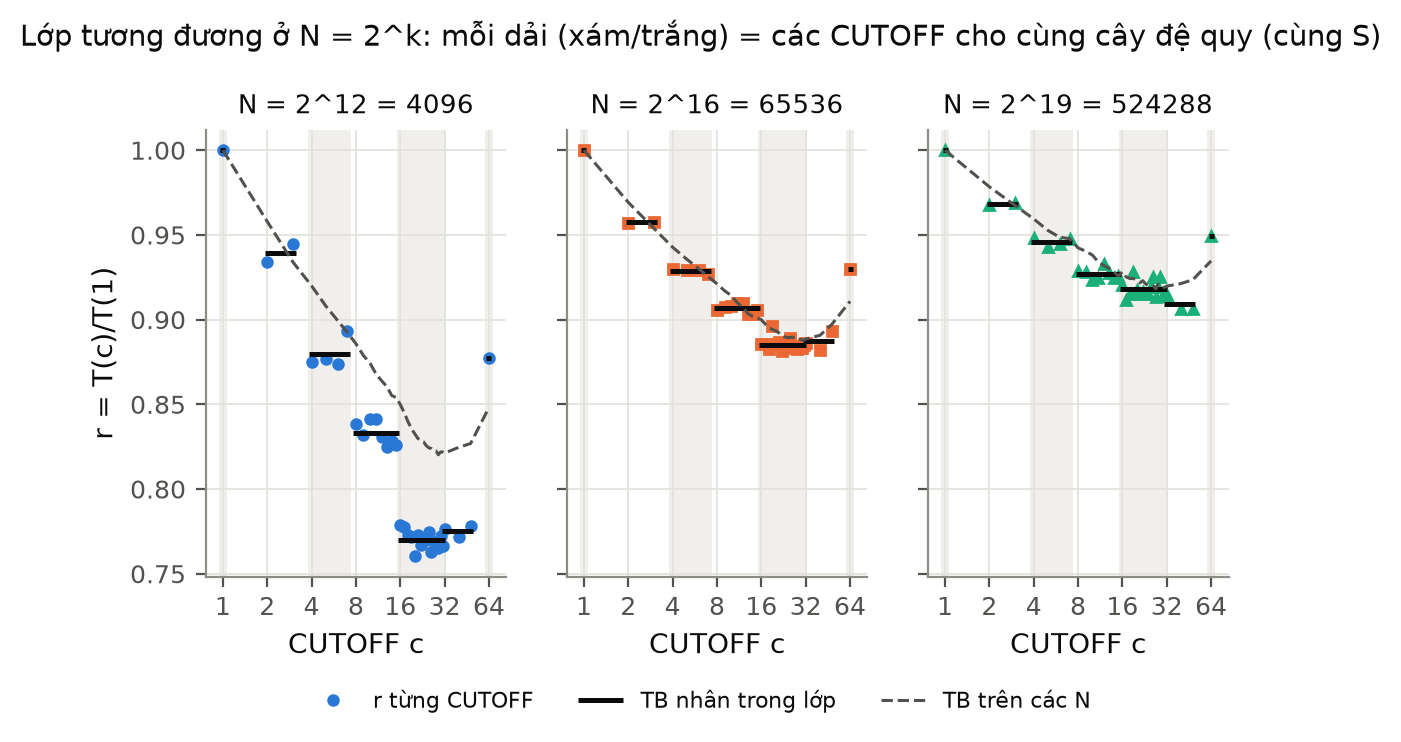
\includegraphics[width=0.95\linewidth]{figures/fig05_equivalence_classes.png}
% Gợi ý chú thích (từ dàn ý): Ở N = 2^k, các CUTOFF trong cùng một dải cho cùng cây đệ quy (cùng S); chênh lệch r trong một dải là nhiễu đo.
\caption{\bv{viết chú thích}}
\label{fig:equiv}
\end{figure}


\subsection{Phương pháp đo}\label{sec:4-3}
% (dàn ý) [F07–F12, F77]
%   - Paired design: mọi CUTOFF dùng chung một mảng gốc; thứ tự CUTOFF được xáo trong mỗi trial.
%   - Thứ tự bộ dữ liệu được xáo theo từng fork.
%   - Mỗi fork là một JVM riêng.
%   - Thủ tục một lần đo: `System.gc()` → clone → bấm giờ → sort → kiểm tra đã sắp.
%   - Lô K: mỗi lô kéo dài ≥ 2 ms; K cố định trong một bộ dữ liệu.
%   - Warm-up: toàn cục cho JVM, và 3 vòng cho mỗi bộ dữ liệu.
%   - Cờ `gc_during_run`.
%   - Lưới CUTOFF và số lần lặp R như thiết kế đã chốt.
%   - **Ghim affinity (chỉ run 3):** [F77, F82]
%     - Cách làm: khởi chạy `run_all.bat` với affinity C00 (LP 10/11 = nhân 5) — ghi đúng lệnh bạn đã dùng (`start /affinity C00`, có `/high` hay không).
%     - Không đổi `Benchmark.java`, dữ liệu, cờ JVM; chỉ đổi cách khởi chạy.
%     - Lý do: chẩn đoán E6 cho thấy luồng đo có thể kẹt trên nhân 0, nơi xung chỉ ở mức sàn ~79% của gói nguồn, và chuyển mức giữa chừng; ghim vào một nhân khác 0 giữ cả lượt ở một mức xung. (mục 7.1; Phụ lục C)
%     - Kiểm chứng: typeperf ghi suốt run 3. [F78]
%     - Ghi rõ: đây là thay đổi quy trình sau khi đã có run 1/2 (xem 7.2).
% BẠN VIẾT:
\bv{Bạn viết nội dung phần này}


\subsection{Phân tích}\label{sec:4-4}
%   - Trung bình nhân của r: log r trung bình trong từng N trước, rồi trung bình trên các N.
%   - CI bootstrap theo cụm N, B = 10 000.
%   - Wilcoxon trên 24 N cộng hiệu chỉnh Holm.
%   - Holdout: chọn c tốt nhất trên các trial lẻ, đánh giá trên các trial chẵn.
%   - Khoảng t qua 9 JVM (3 lượt × 3 fork). (S§2–3, S§9 )
%   - So sánh lượt: Pearson của đường r(c), chênh r tối đa, giao tập gần tối ưu. (S§11 )
% BẠN VIẾT:
\bv{Bạn viết nội dung phần này}


\subsection{Môi trường}\label{sec:4-5}
% (dàn ý) [F13–F15, F82]
%   - Phần cứng, OS, JDK, cờ JVM.
%   - RAM chỉ chạy single-channel.
%   - Chế độ Performance, cắm sạc, không tắt turbo.
%   - Gói nguồn Windows: Balanced; minimum processor state (AC) = 80%.
%   - Đặt vào phụ lục A nếu bảng quá dài.
%
% BẠN VIẾT:
\bv{Bạn viết nội dung phần này}

\begin{table}[H]
\centering
% Gợi ý chú thích (từ dàn ý): Môi trường thí nghiệm.
\caption{\bv{viết chú thích}}
\label{tab:env}
\small
\begin{adjustbox}{max width=\linewidth}% Bảng: môi trường thí nghiệm (results_run3/env_fork1.txt + thông tin máy)
% Sinh tự động bởi report/make_tables.py, KHÔNG sửa tay.
\begin{tabular}{lp{0.75\linewidth}}
\toprule
Thành phần & Cấu hình \\
\midrule
Máy & Lenovo Legion 5 15AHP10 (R7000 AHP10, model 83M0) \\
CPU & AMD Ryzen 7 H 255, 8 nhân / 16 luồng, xung cơ bản 3.8 GHz; L1 512 KB, L2 8 MB (1 MB/nhân), L3 16 MB \\
RAM & 16 GB DDR5-5600, SODIMM, single-channel (1/2 khe) \\
Hệ điều hành & Windows 11 Home 26H2 (build 26300.9711), x64; gói nguồn Balanced \\
JDK & Microsoft OpenJDK 25.0.4.1 (OpenJDK 64-Bit Server VM) \\
Cờ JVM & \texttt{-Xms2g -Xmx2g -XX:+UseSerialGC -XX:+AlwaysPreTouch} \\
Khởi chạy & \texttt{start /b /wait /high}; run 3 thêm \texttt{/affinity C00} (nhân 5) \\
Python & pandas, numpy, scipy, matplotlib (xem \texttt{scripts/requirements.txt}) \\
\bottomrule
\end{tabular}
\end{adjustbox}
\end{table}


\section{Kết quả}\label{sec:5}
%
% BẠN VIẾT:
\bv{Bạn viết nội dung phần này}


\subsection{RQ1: CUTOFF tốt nhất (random)}\label{sec:5-1}
% (dàn ý) [F21–F28]
%   - **Bảng 3:** c tốt nhất, r [CI], vùng gần tối ưu 2% cho từng thang. (S§2; T:rq1_best_cutoff)
%   - **Ý chính 1:** đáy của đường r rất phẳng.
%     - Run 3: vùng 2% rộng 19–48 / 13–48 / 11–64 theo thang. [F21–F23]
%     - Mọi c trong 22–32, 40, 48 nằm trong 2% của c tốt nhất ở cả 3 thang và cả 3 lượt. [F27]
%   - **Ý chính 2:** c tốt nhất theo thang không ổn định giữa các lượt (29/31/27; 31/32/48; 32/29/24), nhưng vùng phẳng thì ổn định. [F24]
%   - Gộp 3 thang: c = 30 (run 3), 31 (run 2), 40 (run 1); cả ba nằm trong vùng phẳng chung. [F25, F26]
%   - **Hình chính: F:fig01.** "Hình 1. Tỉ số thời gian r theo CUTOFF, dữ liệu ngẫu nhiên, ba thang N (trung bình nhân trên 24 N, CI 95% bootstrap theo N)."
%   - **Hình phụ: F:fig02** (phân bố argmin bootstrap) và **F:fig06** (r theo độ dài lá thực tế; r nhỏ nhất ≈ 0.866 ở lá ≈ 17.5). [F28]
% BẠN VIẾT:
\bv{Bạn viết nội dung phần này}

\begin{table}[H]
\centering
% Gợi ý chú thích (từ dàn ý): c tốt nhất, r [CI], vùng gần tối ưu 2% cho từng thang (run 3).
\caption{\bv{viết chú thích}}
\label{tab:rq1}
\small
\begin{adjustbox}{max width=\linewidth}% Bảng: RQ1, dữ liệu ngẫu nhiên, run 3 (T:rq1_best_cutoff)
% Sinh tự động bởi report/make_tables.py, KHÔNG sửa tay.
\begin{tabular}{lccccp{0.2\linewidth}p{0.17\linewidth}}
\toprule
Thang & $c^*$ & $c^*$ (median) & $r$ [CI 95\%] & Giảm & Gần tối ưu ($\le$2\%) & Argmin bootstrap \\
\midrule
$2^{12}$ & 29 & 30 & 0.820 [0.808, 0.831] & 18.0\% & 19--32, 40, 48 & 29: 72\%; 32: 17\%; 30: 8\% \\
$2^{16}$ & 31 & 28 & 0.888 [0.885, 0.890] & 11.2\% & 13--32, 40, 48 & 31: 36\%; 30: 25\%; 32: 20\% \\
$2^{19}$ & 27 & 30 & 0.918 [0.916, 0.920] & 8.2\% & 11--32, 40, 48, 64 & 27: 75\%; 30: 11\%; 31: 9\% \\
\bottomrule
\end{tabular}
\end{adjustbox}
\end{table}

\begin{figure}[H]
\centering
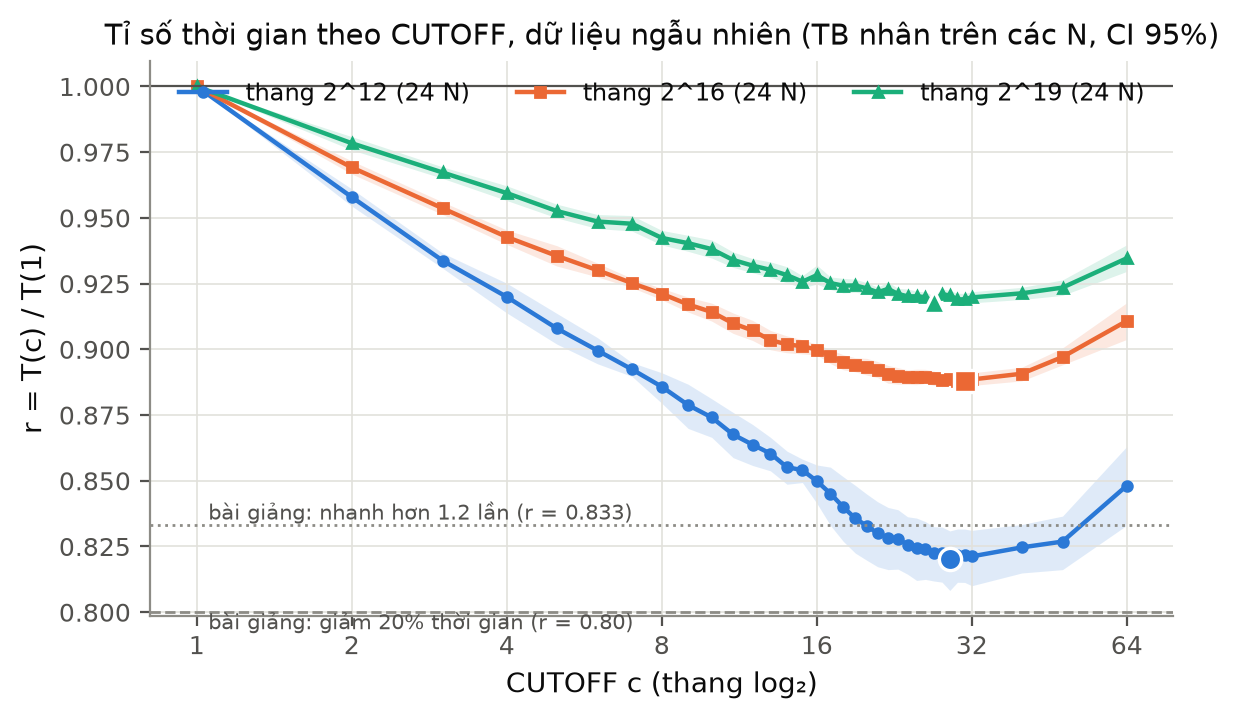
\includegraphics[width=0.95\linewidth]{figures/fig01_r_vs_cutoff_random.png}
% Gợi ý chú thích (từ dàn ý): Tỉ số thời gian r theo CUTOFF, dữ liệu ngẫu nhiên, ba thang N (TB nhân trên 24 N, CI 95% bootstrap theo N).
\caption{\bv{viết chú thích}}
\label{fig:r-cutoff}
\end{figure}

\begin{figure}[H]
\centering
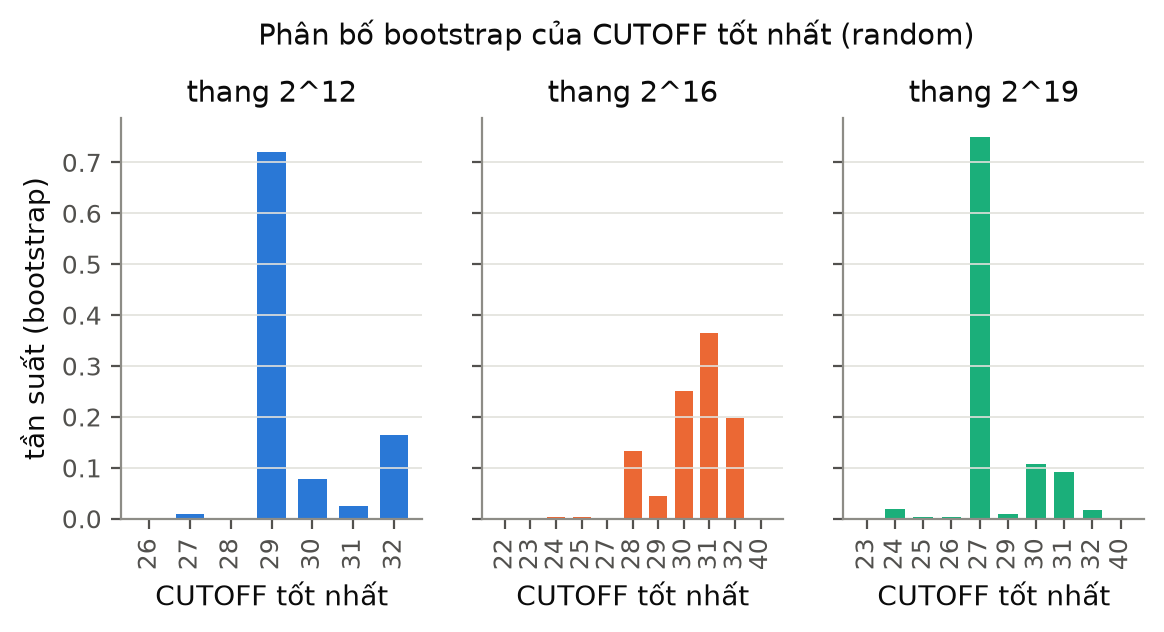
\includegraphics[width=0.85\linewidth]{figures/fig02_argmin_bootstrap.png}
% Gợi ý chú thích (từ dàn ý): Phân bố argmin bootstrap.
\caption{\bv{viết chú thích}}
\label{fig:argmin}
\end{figure}

\begin{figure}[H]
\centering
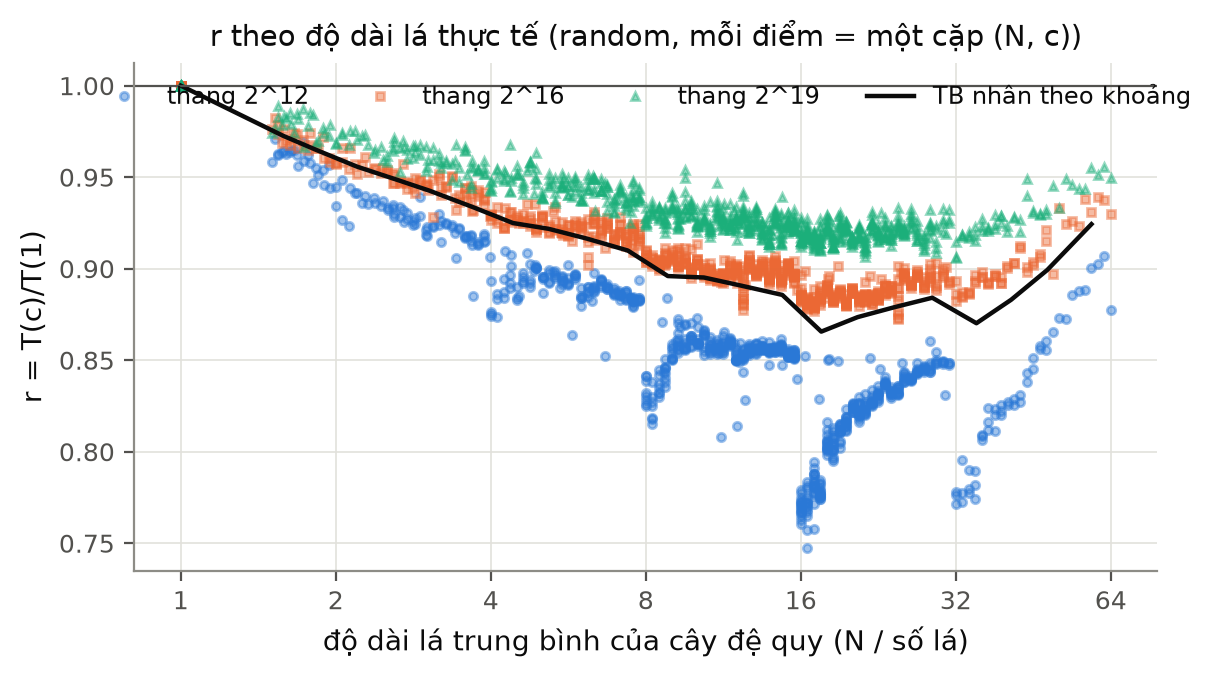
\includegraphics[width=0.85\linewidth]{figures/fig06_r_vs_leaf_length.png}
% Gợi ý chú thích (từ dàn ý): r theo độ dài lá thực tế.
\caption{\bv{viết chú thích}}
\label{fig:leaf}
\end{figure}


\subsection{RQ3: CUTOFF 7, 10 và tốt nhất so với baseline}\label{sec:5-2}
% (dàn ý) [F29–F36]
%   - **Bảng 4:** thời gian giảm [CI] tại c = 7, 10 và c tốt nhất cho 3 thang. (S§3; T:rq3_speedup)
%   - **So với nhận định "20%" của bài giảng:**
%     - Cách đọc r = 0.80: không đạt ở bất kỳ thang nào, ở cả 3 lượt.
%     - Cách đọc 1.2 lần: chỉ đạt ở thang 2^12 với c tốt nhất (1.219×; CI của r nằm dưới 0.833). [F31]
%   - **7 so với 10:** 10 nhanh hơn 7 ở mọi thang và cả 3 lượt; mức chênh 0.9–2.1% (run 3: 1.0–2.1%). Số JVM có 10 nhanh hơn 7:  /9 (S§9). [F33, F34]
%   - **c tốt nhất so với 7 và 10** (holdout): T_best/T_7 = 0.919 / 0.959 / 0.970; T_best/T_10 = 0.940 / 0.972 / 0.981. [F35]
%   - **Hình: F:fig03.** "Hình 3. Mức giảm thời gian tại CUTOFF 7, 10 và tốt nhất; đường đứt: 20% theo bài giảng."
%   - **Hình: F:fig16.** "Hình 4. Biến thiên giữa 9 JVM (3 lượt); dưới: T7/T10 − 1 > 0 nghĩa là 10 nhanh hơn 7."
% BẠN VIẾT:
\bv{Bạn viết nội dung phần này}

\begin{table}[H]
\centering
% Gợi ý chú thích (từ dàn ý): Thời gian giảm [CI] tại c = 7, 10 và c tốt nhất cho 3 thang (run 3).
\caption{\bv{viết chú thích}}
\label{tab:rq3}
\small
\begin{adjustbox}{max width=\linewidth}% Bảng: RQ3, c = 7, 10 và tốt nhất so với c = 1, run 3 (T:rq3_speedup)
% Sinh tự động bởi report/make_tables.py, KHÔNG sửa tay.
\begin{tabular}{llccc}
\toprule
Thang & CUTOFF & $r$ [CI 95\%] & Thời gian giảm [CI 95\%] & Tăng tốc \\
\midrule
$2^{12}$ & $c=7$ & 0.892 [0.890, 0.895] & 10.8\% [10.5\%, 11.0\%] & 1.121$\times$ \\
 & $c=10$ & 0.874 [0.867, 0.881] & 12.6\% [11.9\%, 13.3\%] & 1.144$\times$ \\
 & tốt nhất ($c=29$) & 0.820 [0.808, 0.831] & 18.0\% [16.9\%, 19.2\%] & 1.219$\times$ \\
\addlinespace
$2^{16}$ & $c=7$ & 0.925 [0.923, 0.927] & 7.5\% [7.3\%, 7.7\%] & 1.081$\times$ \\
 & $c=10$ & 0.914 [0.911, 0.918] & 8.6\% [8.2\%, 8.9\%] & 1.094$\times$ \\
 & tốt nhất ($c=31$) & 0.888 [0.885, 0.890] & 11.2\% [11.0\%, 11.5\%] & 1.126$\times$ \\
\addlinespace
$2^{19}$ & $c=7$ & 0.948 [0.945, 0.951] & 5.2\% [4.9\%, 5.5\%] & 1.055$\times$ \\
 & $c=10$ & 0.938 [0.935, 0.942] & 6.2\% [5.8\%, 6.5\%] & 1.066$\times$ \\
 & tốt nhất ($c=27$) & 0.918 [0.916, 0.920] & 8.2\% [8.0\%, 8.4\%] & 1.089$\times$ \\
\bottomrule
\end{tabular}
\end{adjustbox}
\end{table}

\begin{table}[H]
\centering
% Gợi ý chú thích (từ dàn ý): So sánh ghép cặp 7/10 và tốt nhất/7, tốt nhất/10; Wilcoxon trên 24 N, Holm; holdout.
\caption{\bv{viết chú thích}}
\label{tab:paired}
\small
\begin{adjustbox}{max width=\linewidth}% Bảng: so sánh ghép cặp (Wilcoxon trên 24 N, hiệu chỉnh Holm), run 3 (T:rq3_paired_tests)
% Sinh tự động bởi report/make_tables.py, KHÔNG sửa tay.
\begin{tabular}{llcccc}
\toprule
Thang & Loại & $a$ / $b$ & $T_a/T_b$ [CI 95\%] & $a$ nhanh hơn ở & $p$ (Holm) \\
\midrule
$2^{12}$ & in-sample & 7 / 10 & 1.0209 [1.0128, 1.0297] & 3/24 & $5.0\cdot10^{-6}$ \\
$2^{12}$ & in-sample & 29 / 7 & 0.9192 [0.9069, 0.9306] & 24/24 & $2.1\cdot10^{-6}$ \\
$2^{12}$ & in-sample & 29 / 10 & 0.9384 [0.9312, 0.9449] & 24/24 & $2.1\cdot10^{-6}$ \\
$2^{12}$ & holdout & 29 / 7 & 0.9194 [0.9062, 0.9312] & 24/24 & $2.1\cdot10^{-6}$ \\
$2^{12}$ & holdout & 29 / 10 & 0.9397 [0.9322, 0.9470] & 24/24 & $2.1\cdot10^{-6}$ \\
$2^{16}$ & in-sample & 7 / 10 & 1.0120 [1.0079, 1.0162] & 2/24 & $4.0\cdot10^{-5}$ \\
$2^{16}$ & in-sample & 31 / 7 & 0.9597 [0.9575, 0.9621] & 24/24 & $2.1\cdot10^{-6}$ \\
$2^{16}$ & in-sample & 31 / 10 & 0.9713 [0.9685, 0.9740] & 24/24 & $2.1\cdot10^{-6}$ \\
$2^{16}$ & holdout & 28 / 7 & 0.9593 [0.9564, 0.9625] & 24/24 & $2.1\cdot10^{-6}$ \\
$2^{16}$ & holdout & 28 / 10 & 0.9721 [0.9685, 0.9757] & 24/24 & $2.1\cdot10^{-6}$ \\
$2^{19}$ & in-sample & 7 / 10 & 1.0103 [1.0051, 1.0160] & 6/24 & 0.00109 \\
$2^{19}$ & in-sample & 27 / 7 & 0.9687 [0.9650, 0.9720] & 24/24 & $2.1\cdot10^{-6}$ \\
$2^{19}$ & in-sample & 27 / 10 & 0.9786 [0.9756, 0.9817] & 24/24 & $2.1\cdot10^{-6}$ \\
$2^{19}$ & holdout & 27 / 7 & 0.9702 [0.9667, 0.9738] & 24/24 & $2.1\cdot10^{-6}$ \\
$2^{19}$ & holdout & 27 / 10 & 0.9806 [0.9769, 0.9844] & 23/24 & $2.1\cdot10^{-6}$ \\
\bottomrule
\end{tabular}
\end{adjustbox}
\end{table}

\begin{figure}[H]
\centering
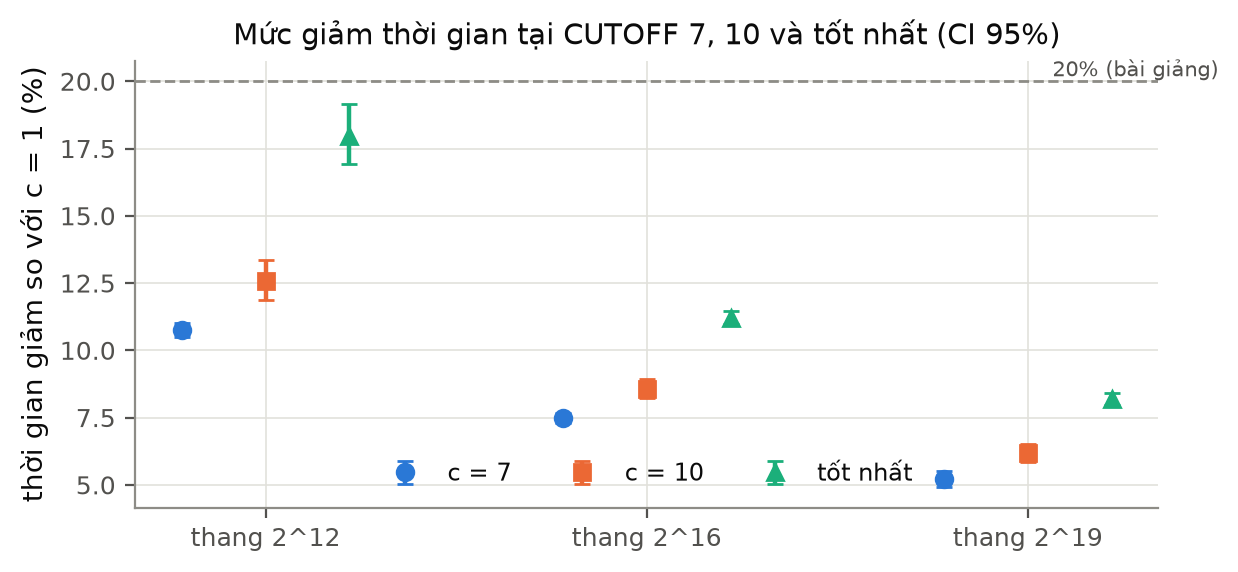
\includegraphics[width=0.95\linewidth]{figures/fig03_speedup_7_10_best.png}
% Gợi ý chú thích (từ dàn ý): Mức giảm thời gian tại CUTOFF 7, 10 và tốt nhất; đường đứt: 20% theo bài giảng.
\caption{\bv{viết chú thích}}
\label{fig:speedup}
\end{figure}

\begin{figure}[H]
\centering
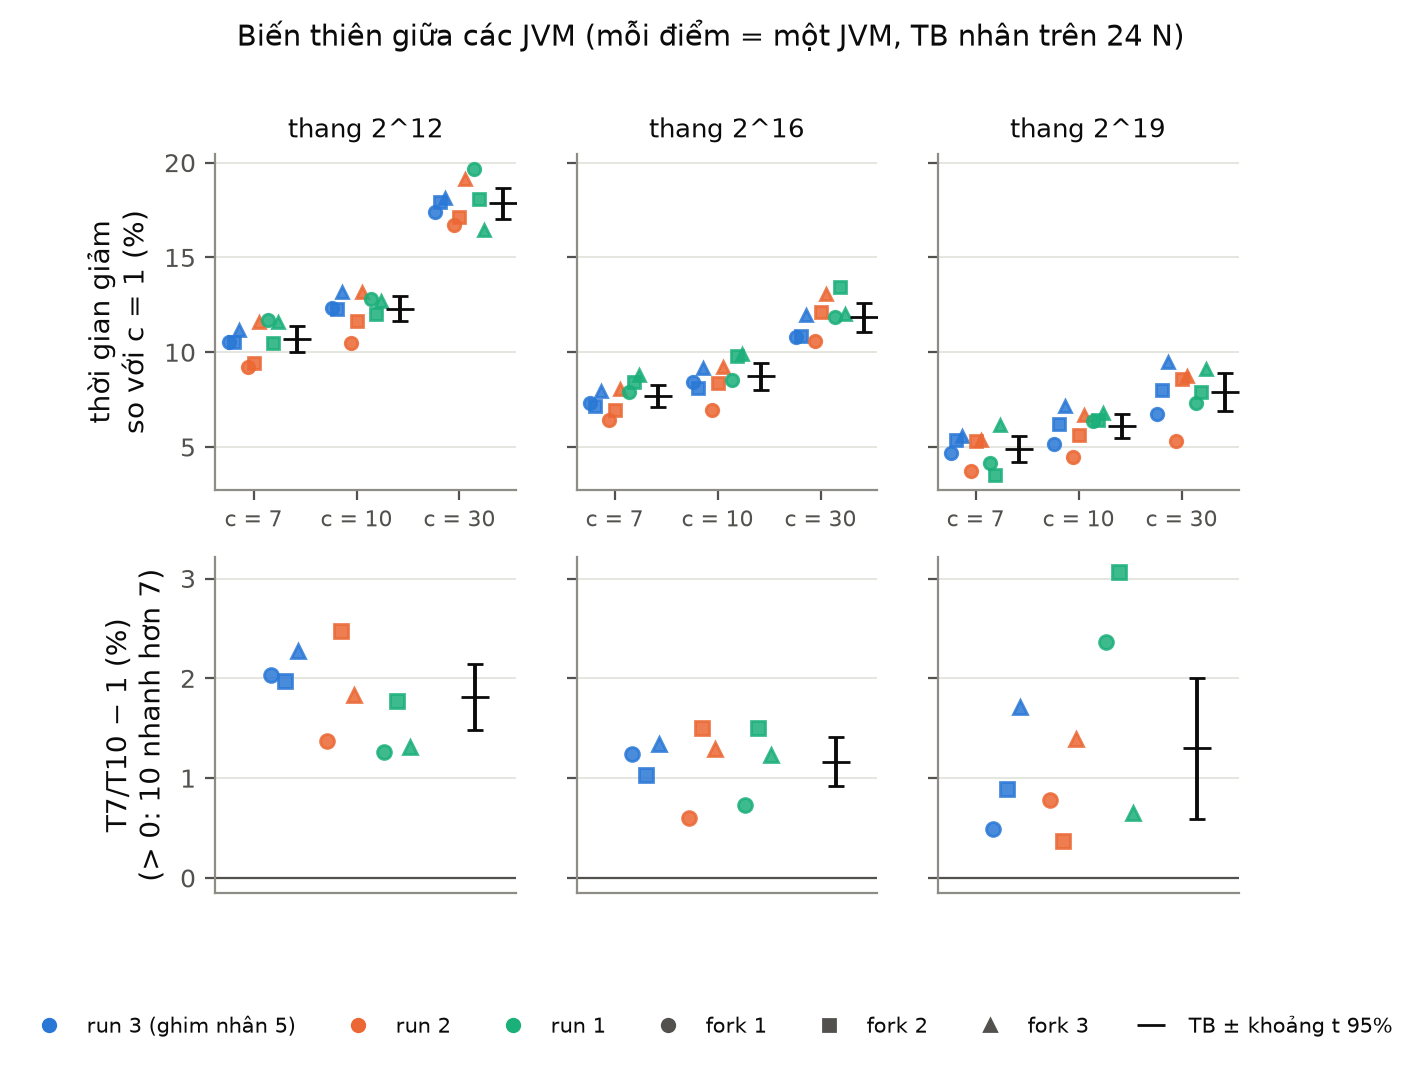
\includegraphics[width=0.95\linewidth]{figures/fig16_per_jvm.png}
% Gợi ý chú thích (từ dàn ý): Biến thiên giữa 9 JVM (3 lượt); dưới: T7/T10 − 1 > 0 nghĩa là 10 nhanh hơn 7.
\caption{\bv{viết chú thích}}
\label{fig:perjvm}
\end{figure}


\subsection{RQ2: ảnh hưởng của N và phân bố}\label{sec:5-3}
% (dàn ý) [F37–F43]
%   - **Theo N:** mức giảm lớn nhất giảm dần khi N tăng: 18.0% → 11.2% → 8.2%.
%   - **Theo phân bố (thang 2^16):** **Bảng 5** gồm c tốt nhất, thời gian giảm và vùng gần tối ưu. (S§5)
%     - Đảo ngược: tốt nhất 8 ở run 3, 10 ở run 2/1; cả hai nằm trong vùng chung 6–12. [F40, F42]
%   - **Hình: F:fig08.** "Hình 5. r theo CUTOFF cho 5 phân bố (thang 2^16); marker lớn là CUTOFF tốt nhất."
%   - **Hình phụ: F:fig07.** "Heatmap N × CUTOFF."
% BẠN VIẾT:
\bv{Bạn viết nội dung phần này}

\begin{table}[H]
\centering
% Gợi ý chú thích (từ dàn ý): c tốt nhất, thời gian giảm và vùng gần tối ưu theo phân bố (thang 2^16, run 3).
\caption{\bv{viết chú thích}}
\label{tab:dist}
\small
\begin{adjustbox}{max width=\linewidth}% Bảng: các phân bố, thang 2^16, run 3 (T:rq1_best_cutoff)
% Sinh tự động bởi report/make_tables.py, KHÔNG sửa tay.
\begin{tabular}{lcccp{0.3\linewidth}}
\toprule
Phân bố & $c^*$ & $r$ [CI 95\%] & Giảm & Gần tối ưu ($\le$2\%) \\
\midrule
ngẫu nhiên & 31 & 0.888 [0.885, 0.890] & 11.2\% & 13--32, 40, 48 \\
đã sắp & 64 & 0.647 [0.642, 0.651] & 35.3\% & 64 \\
đảo ngược & 8 & 0.887 [0.884, 0.890] & 11.3\% & 6, 8, 10, 12 \\
gần sắp (\textasciitilde 1\%) & 64 & 0.686 [0.682, 0.689] & 31.4\% & 64 \\
ít giá trị (10) & 32 & 0.828 [0.825, 0.830] & 17.2\% & 20, 24, 32, 48 \\
\bottomrule
\end{tabular}
\end{adjustbox}
\end{table}

\begin{figure}[H]
\centering
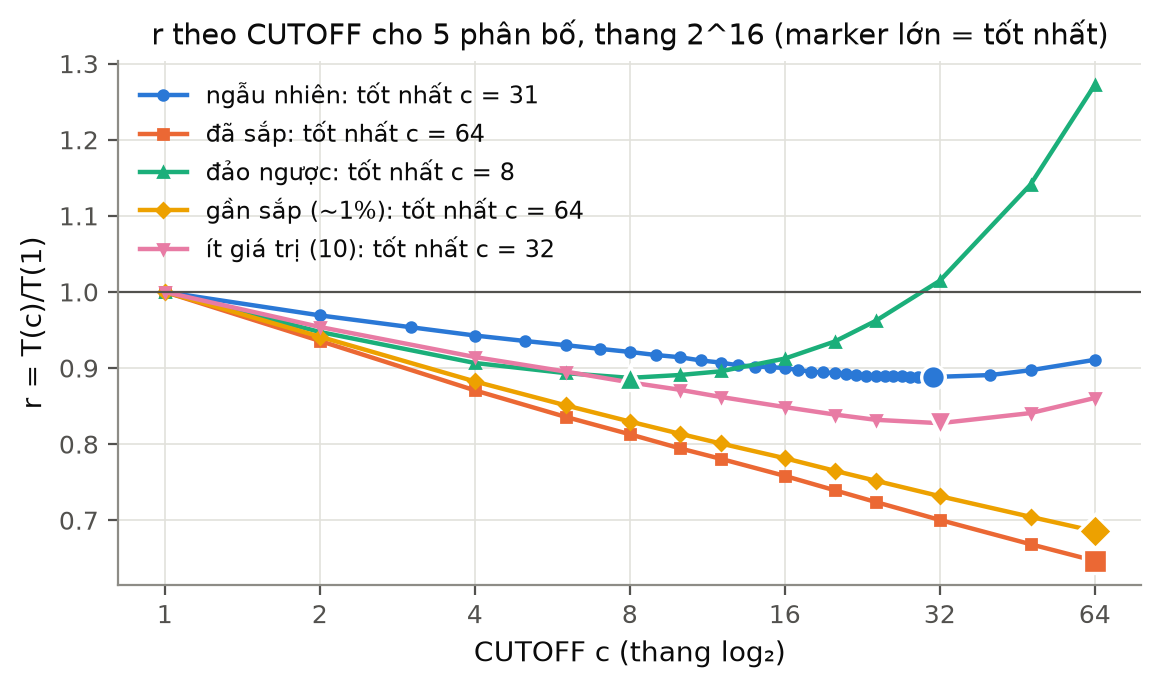
\includegraphics[width=0.95\linewidth]{figures/fig08_distributions_2e16.png}
% Gợi ý chú thích (từ dàn ý): r theo CUTOFF cho 5 phân bố (thang 2^16); marker lớn là CUTOFF tốt nhất.
\caption{\bv{viết chú thích}}
\label{fig:dist}
\end{figure}

\begin{figure}[H]
\centering
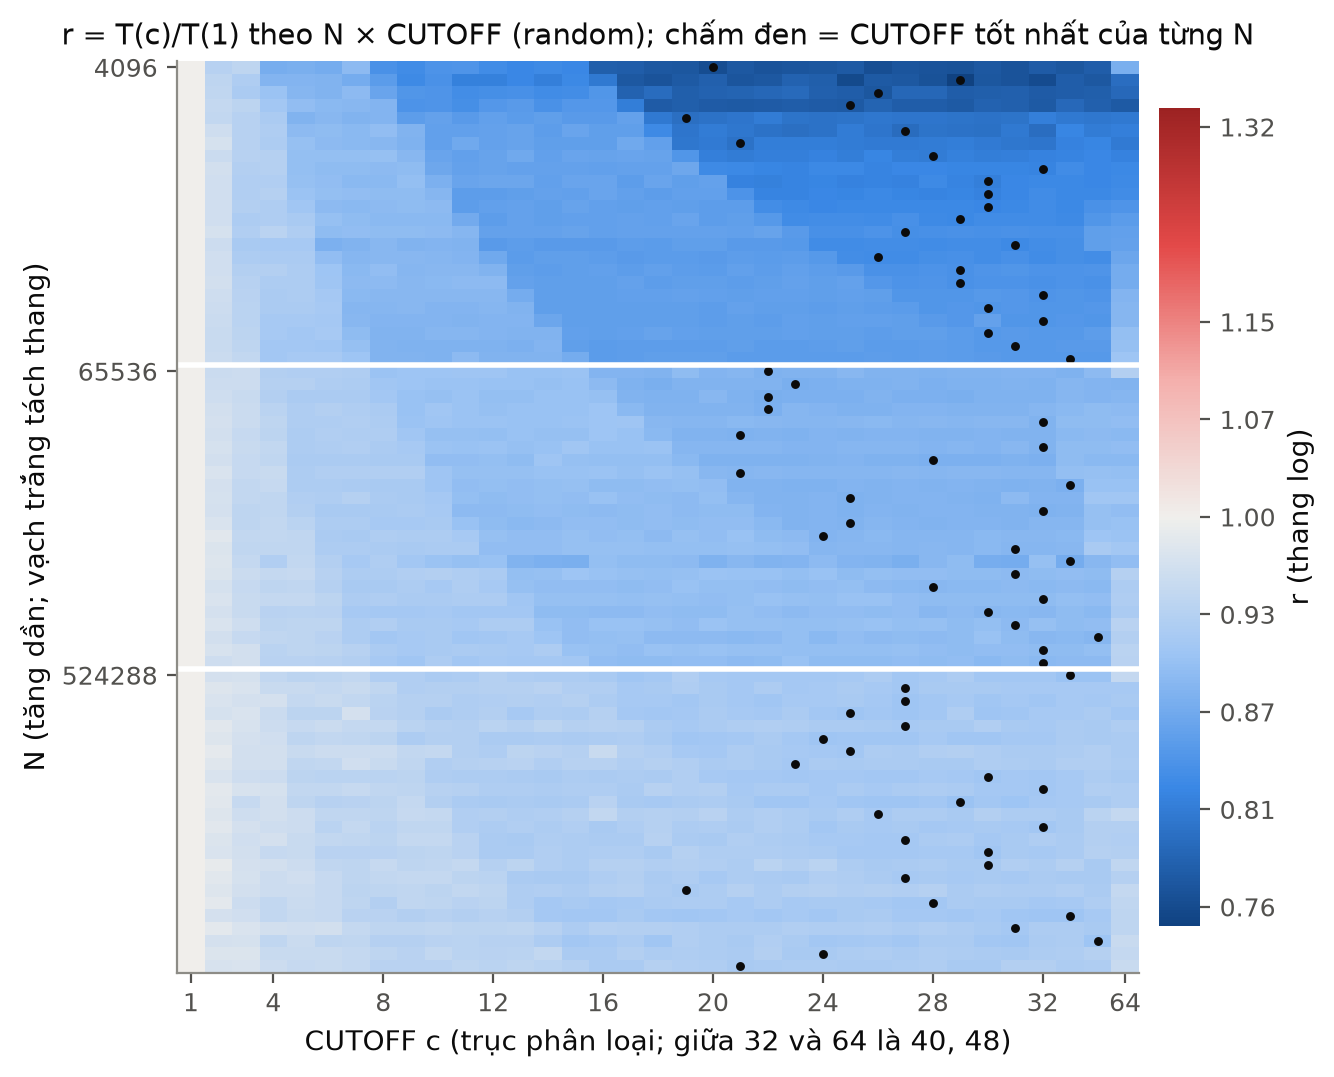
\includegraphics[width=0.85\linewidth]{figures/fig07_heatmap_random.png}
% Gợi ý chú thích (từ dàn ý): Heatmap N × CUTOFF.
\caption{\bv{viết chú thích}}
\label{fig:heatmap}
\end{figure}


\subsection{Số đếm}\label{sec:5-4}
% (dàn ý) [F44–F48]
%   - Ở c tốt nhất: C tăng, A tăng nhẹ, S giảm, trong khi T giảm. (S§6; T:counts_normalized)
%   - Ở c = 1, các số đếm khớp cận trong bài giảng.
%   - **Hình: F:fig09.** "Hình 6. Số đếm và thời gian theo CUTOFF (tỉ số so với c = 1)."
% BẠN VIẾT:
\bv{Bạn viết nội dung phần này}

\begin{figure}[H]
\centering
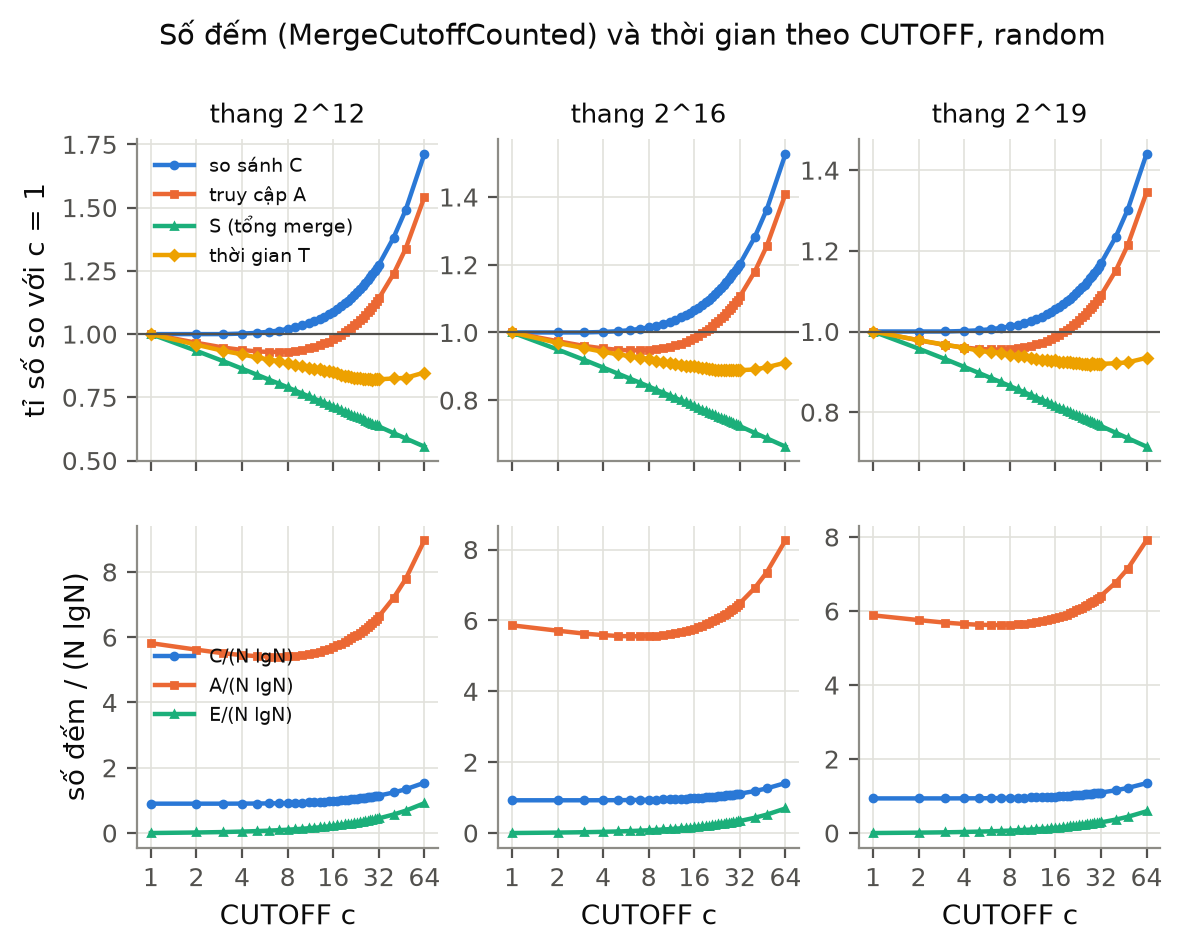
\includegraphics[width=0.95\linewidth]{figures/fig09_counts_vs_time.png}
% Gợi ý chú thích (từ dàn ý): Số đếm và thời gian theo CUTOFF (tỉ số so với c = 1).
\caption{\bv{viết chú thích}}
\label{fig:counts}
\end{figure}


\subsection{Mô hình thời gian chạy}\label{sec:5-5}
% (dàn ý) [F49–F55]
%   - T = a·N^b: b = 1.151 (c = 1) và 1.175 (c = 30), trong khi N lgN thuần trên cùng tập N cho b = 1.092.
%   - Mô hình k·N lgN khớp từ 2^12 và 2^16 dự đoán thấp hơn thực tế khoảng 20–26% ở 2^19; power law chỉ lệch −3.7% / −0.9%. (S§7)
%   - **Hình: F:fig10.** Mô hình thời gian.
%   - **Hình: F:fig14.** "Hình 7. T/(N lgN) theo N; vạch dọc: working set 24N byte bằng dung lượng L2 và L3."
%   - Giới hạn cách diễn giải: xem mục 6 và 7.
% BẠN VIẾT:
\bv{Bạn viết nội dung phần này}

\begin{table}[H]
\centering
% Gợi ý chú thích (từ dàn ý): Mô hình T = a·N^b (run 3).
\caption{\bv{viết chú thích}}
\label{tab:model}
\small
\begin{adjustbox}{max width=\linewidth}% Bảng: mô hình T = a N^b, random, run 3 (T:runtime_model)
% Sinh tự động bởi report/make_tables.py, KHÔNG sửa tay.
\begin{tabular}{cccccc}
\toprule
CUTOFF & Số N & $b$ & $a$ (ns) & $R^2$ & $T/(N\lg N)$ (ns) \\
\midrule
1 & 72 & 1.1509 $\pm$ 0.0020 & 28.34 & 0.99980 & 9.664 \\
30 & 72 & 1.1746 $\pm$ 0.0027 & 19.04 & 0.99962 & 8.459 \\
\bottomrule
\end{tabular}
\end{adjustbox}
\end{table}

\begin{figure}[H]
\centering
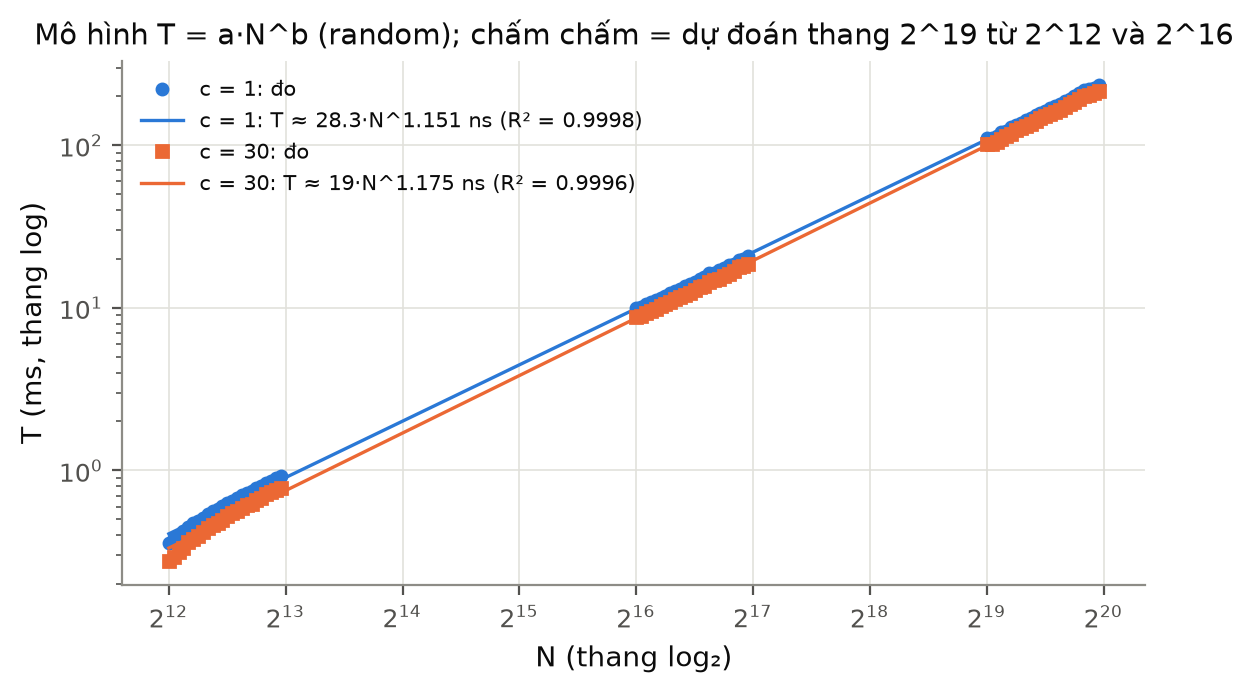
\includegraphics[width=0.95\linewidth]{figures/fig10_runtime_model.png}
% Gợi ý chú thích (từ dàn ý): Mô hình thời gian chạy.
\caption{\bv{viết chú thích}}
\label{fig:model}
\end{figure}

\begin{figure}[H]
\centering
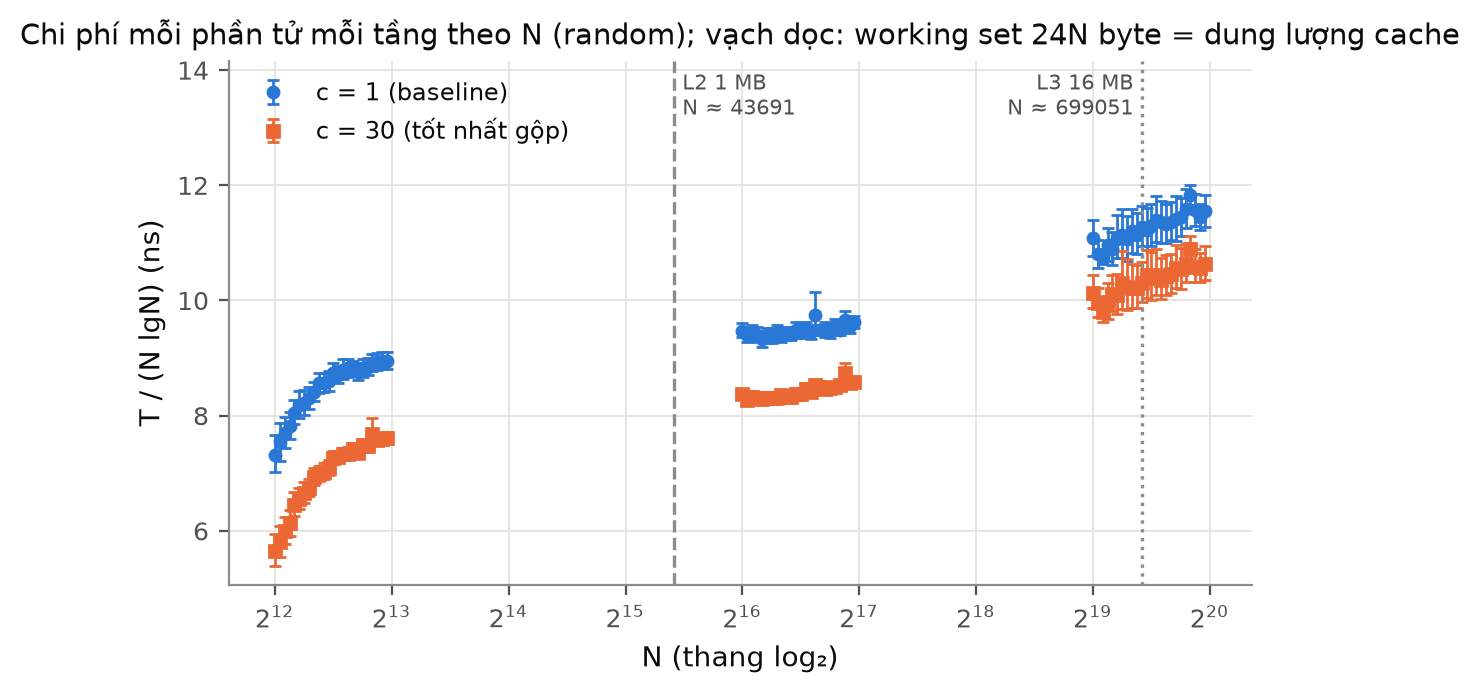
\includegraphics[width=0.95\linewidth]{figures/fig14_cache_levels.png}
% Gợi ý chú thích (từ dàn ý): T/(N lgN) theo N; vạch dọc: working set 24N byte bằng dung lượng L2 và L3.
\caption{\bv{viết chú thích}}
\label{fig:cache}
\end{figure}


\subsection{Độ lặp lại qua 3 lượt}\label{sec:5-6}
% (dàn ý) [F56, F27, F42, F84]
%   - **Bảng 6 (3 lượt, random):** theo thang: c tốt nhất, vùng gần tối ưu, giao 3 lượt, giảm tại 7 / 10 / tốt nhất, T7/T10 (p), T/(N lgN) c = 1 so với run 3. (S§11 ; T:compare_best, T:compare_near_intersection)
%   - **Bảng 7 (từng cặp lượt):** Pearson của r(c) và chênh r tối đa, cho mọi (phân bố, thang). (S§11 ; T:compare_pairs)
%   - Ý chính:
%     - Thời gian tuyệt đối khác nhau 1.79–1.87 lần (run 2 so với run 3), nhưng r gần như trùng. [F56, F84]
%     - Vùng gần tối ưu của run 3 chứa trọn vùng của run 2 ở cả 3 thang, nên giao 3 lượt = giao của run 1 và run 2. [F27]
%   - **Hình: F:fig15.** "Hình 8. r theo CUTOFF ở 3 lượt (trên) và r của từng lượt so với lượt chính (dưới)."
%
% BẠN VIẾT:
\bv{Bạn viết nội dung phần này}

\begin{table}[H]
\centering
% Gợi ý chú thích (từ dàn ý): 3 lượt, random: c tốt nhất, vùng gần tối ưu, giao 3 lượt, giảm tại 7/10/tốt nhất, T7/T10, T/(N lgN) ở c = 1.
\caption{\bv{viết chú thích}}
\label{tab:runs}
\small
\begin{adjustbox}{max width=\linewidth}% Bảng: 3 lượt, random (T:compare_best, T:compare_near_intersection)
% Sinh tự động bởi report/make_tables.py, KHÔNG sửa tay.
\begin{tabular}{llcp{0.17\linewidth}cccccc}
\toprule
Thang & Lượt & $c^*$ & Gần tối ưu & Giảm $c{=}7$ & Giảm $c{=}10$ & Giảm $c^*$ & $T_7/T_{10}$ & $p_{7\,\mathrm{vs}\,10}$ & $T/(N\lg N)$, $c{=}1$ (ns) \\
\midrule
$2^{12}$ & run 3 & 29 & 19--32, 40, 48 & 10.8\% & 12.6\% & 18.0\% & 1.0209 & $1.7\cdot10^{-6}$ & 8.46 \\
 & run 2 & 31 & 22--32, 40, 48 & 10.1\% & 11.8\% & 17.9\% & 1.0189 & $9.6\cdot10^{-4}$ & 15.82 \\
 & run 1 & 32 & 21--32, 40, 48 & 11.3\% & 12.5\% & 18.2\% & 1.0145 & 0.0315 & 16.56 \\
 & \multicolumn{9}{l}{\textit{giao 3 lượt:} 22--32, 40, 48} \\
\addlinespace
$2^{16}$ & run 3 & 31 & 13--32, 40, 48 & 7.5\% & 8.6\% & 11.2\% & 1.0120 & $2.0\cdot10^{-5}$ & 9.48 \\
 & run 2 & 32 & 19--32, 40, 48 & 7.2\% & 8.2\% & 12.0\% & 1.0113 & $1.8\cdot10^{-4}$ & 16.99 \\
 & run 1 & 29 & 18--32, 40, 48 & 8.4\% & 9.4\% & 12.7\% & 1.0115 & 0.00434 & 18.21 \\
 & \multicolumn{9}{l}{\textit{giao 3 lượt:} 19--32, 40, 48} \\
\addlinespace
$2^{19}$ & run 3 & 27 & 11--32, 40, 48, 64 & 5.2\% & 6.2\% & 8.2\% & 1.0103 & 0.00109 & 11.26 \\
 & run 2 & 48 & 12--32, 40, 48, 64 & 4.8\% & 5.6\% & 7.9\% & 1.0085 & 0.0269 & 20.49 \\
 & run 1 & 24 & 11, 13, 15--32, 40, 48, 64 & 4.6\% & 6.5\% & 8.8\% & 1.0202 & 0.00434 & 20.54 \\
 & \multicolumn{9}{l}{\textit{giao 3 lượt:} 13, 15--32, 40, 48, 64} \\
\bottomrule
\end{tabular}
\end{adjustbox}
\end{table}

\begin{table}[H]
\centering
% Gợi ý chú thích (từ dàn ý): 3 lượt, các phân bố khác (thang 2^16).
\caption{\bv{viết chú thích}}
\label{tab:runs-other}
\small
\begin{adjustbox}{max width=\linewidth}% Bảng: 3 lượt, các phân bố khác (T:compare_best)
% Sinh tự động bởi report/make_tables.py, KHÔNG sửa tay.
\begin{tabular}{lcccl}
\toprule
Phân bố ($2^{16}$) & run 3: $c^*$ ($r$) & run 2 & run 1 & Giao vùng gần tối ưu \\
\midrule
đã sắp & 64 (0.647) & 64 (0.664) & 64 (0.653) & 64 \\
đảo ngược & 8 (0.887) & 10 (0.890) & 10 (0.885) & 6, 8, 10, 12 \\
gần sắp (\textasciitilde 1\%) & 64 (0.686) & 64 (0.701) & 64 (0.703) & 64 \\
ít giá trị (10) & 32 (0.828) & 32 (0.816) & 32 (0.813) & 24, 32, 48 \\
\bottomrule
\end{tabular}
\end{adjustbox}
\end{table}

\begin{table}[H]
\centering
% Gợi ý chú thích (từ dàn ý): Pearson của r(c) và chênh r tối đa giữa từng cặp lượt.
\caption{\bv{viết chú thích}}
\label{tab:pairs}
\small
\begin{adjustbox}{max width=\linewidth}% Bảng: Pearson của r(c) (chênh r tối đa) giữa từng cặp lượt (T:compare_pairs)
% Sinh tự động bởi report/make_tables.py, KHÔNG sửa tay.
\begin{tabular}{llccc}
\toprule
Phân bố & Thang & run 3 -- run 2 & run 3 -- run 1 & run 2 -- run 1 \\
\midrule
ngẫu nhiên & $2^{12}$ & 0.998 (1.20\%) & 0.996 (0.92\%) & 0.997 (1.27\%) \\
ngẫu nhiên & $2^{16}$ & 0.986 (0.97\%) & 0.980 (2.09\%) & 0.991 (1.53\%) \\
ngẫu nhiên & $2^{19}$ & 0.981 (1.04\%) & 0.946 (1.57\%) & 0.962 (1.17\%) \\
đã sắp & $2^{16}$ & 1.000 (2.72\%) & 0.999 (1.64\%) & 1.000 (1.69\%) \\
đảo ngược & $2^{16}$ & 0.998 (3.43\%) & 0.998 (4.82\%) & 0.998 (2.31\%) \\
gần sắp (\textasciitilde 1\%) & $2^{16}$ & 0.999 (2.45\%) & 0.999 (2.59\%) & 0.999 (0.96\%) \\
ít giá trị (10) & $2^{16}$ & 0.987 (1.57\%) & 0.987 (2.12\%) & 0.998 (0.93\%) \\
\bottomrule
\end{tabular}
\end{adjustbox}
\end{table}

\begin{figure}[H]
\centering
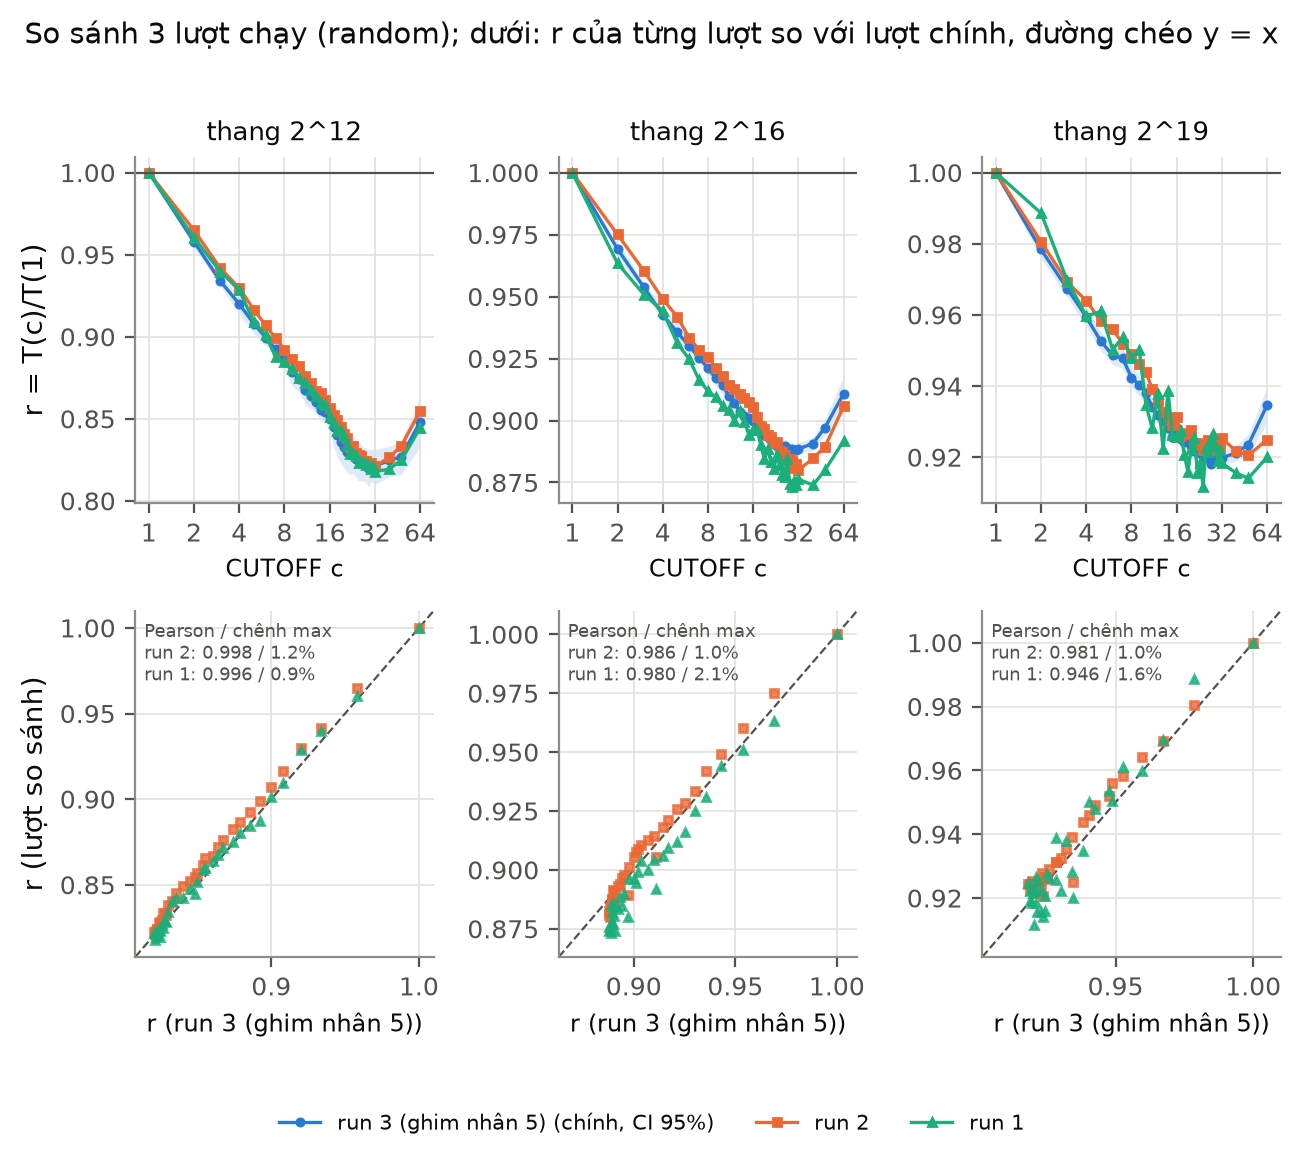
\includegraphics[width=0.95\linewidth]{figures/fig15_run_comparison.png}
% Gợi ý chú thích (từ dàn ý): r theo CUTOFF ở 3 lượt (trên) và r của từng lượt so với lượt chính (dưới).
\caption{\bv{viết chú thích}}
\label{fig:runs}
\end{figure}


\section{Thảo luận}\label{sec:6}
%
% - **Vì sao mức giảm nhỏ dần khi N tăng**
%   - Cutoff bỏ khoảng lg(lá) tầng đáy trong tổng khoảng lg N tầng.
%   - Phần merge bị bỏ ở c tốt nhất (29 / 31 / 27) là 35% / 27% / 22%, trong khi thời gian chỉ giảm 18.0% / 11.2% / 8.2%. [F44, F46]
%   - Gợi ý ý: các tầng đáy rẻ hơn tính trên mỗi phần tử, vì nằm gọn trong cache; ở N lớn, các tầng trên (tốn bộ nhớ) chiếm tỉ trọng thời gian lớn hơn. Liên hệ với F:fig14, nhưng chỉ ở mức "phù hợp với".
% - **Vì sao C tăng mà T giảm**
%   - Số liệu: C ×1.237, A ×1.108, S ×0.646, T ×0.820 (2^12, c = 29). [F44]
%   - Gợi ý ý: chi phí của một phép so sánh hoặc truy cập không giống nhau.
%     - Insertion sort chạy trên đoạn nhỏ, liền kề, nằm trong L1, không có lời gọi đệ quy và không copy sang `aux`.
%     - Vì vậy mô hình "đếm phép toán" của bài giảng chưa đủ để dự đoán thời gian.
%   - Có thể nhắc thêm: ở c = 7, A còn giảm (×0.929) dù C tăng (×1.014). [F45]
% - **Vì sao đảo ngược tối ưu quanh 8–10, còn đã sắp tối ưu ở đầu mút lưới**
%   - Lá đảo ngược là trường hợp xấu nhất của insertion sort: k(k−1)/2 so sánh và đổi chỗ. r tăng mạnh khi lá lớn (run 2: 0.990 / 1.102 / 1.239 tại c = 32 / 48 / 64; run 3:  T:r_by_cutoff). [F40]
%   - Lá đã sắp chỉ tốn tuyến tính (k − 1 so sánh, 0 đổi chỗ), nên r giảm đơn điệu đến 64. Tối ưu thật có thể > 64, chưa xác định được vì nằm ngoài lưới. [F37]
%   - Gần sắp cũng tối ưu ở 64; ít giá trị tối ưu ở 32, tương tự random.
% - **7 so với 10**
%   - Ở N = 2^k, đây là so sánh "lá 4" với "lá 8".
%   - 10 thắng nhưng chỉ khoảng 1–2%; cả hai đều cách xa vùng 22–48. [F33, F34, F35]
%   - Gợi ý ý: con số trong sách gắn với máy, ngôn ngữ và kiểu dữ liệu cụ thể; không nên coi là hằng số.
% - **Vì sao không đạt 20%**
%   - Bài giảng chỉ nói "có thể... khoảng 20%".
%   - Ở đây chỉ đạt theo cách đọc 1.2 lần, ở 2^12, với c tốt nhất. [F31]
%   - Các ý có thể bàn, dưới dạng giả thuyết chứ không khẳng định:
%     - `Integer[]` với `compareTo` gọi qua interface và qua tham chiếu làm mỗi phép so sánh đắt, trong khi insertion sort tăng C.
%     - Hiệu ứng bộ nhớ ở N lớn làm loãng phần lợi.
%     - Bài giảng có thể đo ở N, máy hoặc ngôn ngữ khác.
%   - Mức xung không phải lý do: run 3 (xung cao) cho mức giảm gần như bằng run 2 (xung thấp). (ý tiếp theo)
% - **r gần như không đổi giữa hai mức xung** [F56, F78, F84]
%   - Hai điều kiện: run 3 (nhân 5, ~129% ≈ 4.9 GHz, đo bằng typeperf) và run 2 (suy ra: nhân 0, ~79% ≈ 3.0 GHz).
%   - Thời gian tuyệt đối khác 1.79–1.87 lần; r: Pearson 0.981–0.998, chênh tối đa ≤ 1.2% (random); mức giảm tại 7 / 10 / tốt nhất chênh ≤ 0.8 điểm %; 7 so với 10 cùng chiều.
%   - Gợi ý ý: cutoff thay đổi lượng công việc (S, C, A, số lời gọi), mà các phần công việc này co giãn gần như cùng tỉ lệ theo xung, nên tỉ số r gần như giữ nguyên.
%   - Giới hạn của ý này: hai điều kiện khác nhau cả về nhân (nhân 0 có thêm phần phạt ngoài xung, xem T2 [F81]), chứ không chỉ về xung. Nên viết "r bền qua hai điều kiện xung/nhân", không viết "r độc lập với xung".
% - **Hiệu ứng bộ nhớ ở xung cao** [F51–F53]
%   - Rõ hơn ở run 3 trong thang 2^19:
%     - Quanh ngưỡng L3: dưới / trên = 11.01 / 11.43 ns (+3.8%), so với 20.57 / 20.44 (−0.6%) ở run 2.
%     - Xu hướng trong thang 2^19: +7.5% mỗi lần gấp đôi N, so với −2.5% ở run 2.
%   - Gợi ý ý: độ trễ DRAM cố định theo ns; khi nhân chạy nhanh, phần tính toán co lại nên phần chờ bộ nhớ chiếm tỉ trọng lớn hơn.
%   - Không đồng nhất, nên viết thận trọng:
%     - Tỉ số 2^19:2^16 của run 3 (1.188) không lớn hơn run 2 (1.206).
%     - Xu hướng trong thang 2^12 cũng khác mạnh (+20.0% so với +5.6%), dù dữ liệu 2^12 nằm trong L2, mà L1/L2 chạy theo xung nhân. Độ trễ DRAM không giải thích được phần này.
% - **Độ tin cậy của kết luận**
%   - Ba lượt cho r gần như trùng nhau (Bảng 7). [F56]
%   - Kết luận "vùng phẳng 22–32, 40, 48" và "10 tốt hơn 7" bền qua cả 3 lượt và 2 mức xung.
%
% BẠN VIẾT:
\bv{Bạn viết nội dung phần này}


\section{Hạn chế}\label{sec:7}
%
% BẠN VIẾT:
\bv{Bạn viết nội dung phần này}


\subsection{Hai mức hiệu năng ("bước nhảy"): luồng đo kẹt trên nhân 0 ở xung thấp}\label{sec:7-1}
% (dàn ý) [F57–F63, F65–F84]
%   - Hiện tượng (run 1/2, pilot):
%     - Cả 6 JVM của run 1/2 nhảy lên mức chậm ở vòng warm-up 5–7 (1.14–1.68×) và giữ mức đó suốt khoảng 45 phút. [F57]
%     - Pilot chuyển qua lại giữa hai mức trong lúc đo. [F59, F65]
%   - Chuỗi chẩn đoán (chi tiết ở Phụ lục C):
%     1. PrintCompilation: không có sự kiện biên dịch nào quanh lúc chuyển mức → loại JIT. [F66–F68]
%     2. E0_1 / E0_2 (WarmupProbe + typeperf): 296/300 và 900/900 vòng nhanh; 4 vòng chậm trùng lúc luồng sang LP 1 (nhân 0). [F71, F72]
%     3. E6 (Benchmark như `run_all.bat` + typeperf): giai đoạn chậm = luồng trên nhân 0 ở 77–79%; giai đoạn nhanh trên nhân 5/7 ở 125–128%. [F74–F76]
%     4. T2 (Benchmark ghim nhân 0 / nhân 5): khi bị ghim, nhân 0 vẫn boost tới 123.6–127% → không phải giới hạn phần cứng. Mức 79% ≈ minimum processor state 80% của gói nguồn. [F81, F82]
%     5. Run 3 (ghim nhân 5, cả lượt + typeperf): 100% mẫu trên nhân 5, xung 128–129.5%, không có bước nhảy. [F77, F78, F83]
%   - Đã xác định:
%     - Mức chậm = luồng đo chạy trên nhân 0 trong khi nhân này ở mức xung sàn (đo trực tiếp ở E6).
%     - Không do JIT, không do tiến trình khác, không do SMT, không do giới hạn phần cứng của nhân 0.
%     - Run 3 nằm trọn ở mức nhanh.
%   - Chưa rõ:
%     - Vì sao Windows giữ nhân 0 ở mức sàn khi có luồng bận (E6, có lẽ cả run 1/2), nhưng lại boost khi tiến trình bị ghim vào nhân 0 (T2). Giả thuyết: chính sách điện năng / lập lịch của Windows hoặc firmware; chưa kiểm tra.
%     - Vì sao luồng của Benchmark ở lại nhân 0 lâu (2 phút ở E6; nhiều khả năng 45 phút ở run 1/2), còn WarmupProbe rời đi sau vài giây.
%     - Run 1/2 không có typeperf: "kẹt trên nhân 0 suốt lượt" là giải thích phù hợp nhất (cùng kiểu nhảy, cùng tỉ lệ) nhưng **chưa đo trực tiếp**.
%     - Phần dư: thời gian run 2 : run 3 = 1.79–1.87, lớn hơn tỉ lệ xung 1.62. T2 cho thấy nhân 0 chậm hơn nhân 5 thêm khoảng 2–6% (2^16) đến 18–32% (2 bộ 2^19) sau khi đã trừ chênh xung (~2%); mỗi điều kiện chỉ đo 1 lần, nguyên nhân chưa rõ. [F81, F84]
%   - Hệ quả cho kết quả:
%     - Mỗi lượt nằm trọn ở một mức (run 3: không chuyển mức; run 1/2: không chuyển mức sau warm-up), nên r trong mỗi lượt nhất quán.
%     - Thời gian tuyệt đối và T/(N lgN) phụ thuộc mức; báo cáo theo run 3.
%     - r bền qua hai mức (mục 6).
%   - Ước lượng của pilot thấp hơn thời gian thực của run 1/2 (1:17:48 và 1:40:01, so với 2:16:48 và 2:13:12), vì pilot chủ yếu chạy ở mức nhanh; run 3 (1:15:21) khớp với mức nhanh. [F63, F77]
% BẠN VIẾT:
\bv{Bạn viết nội dung phần này}

\begin{figure}[H]
\centering
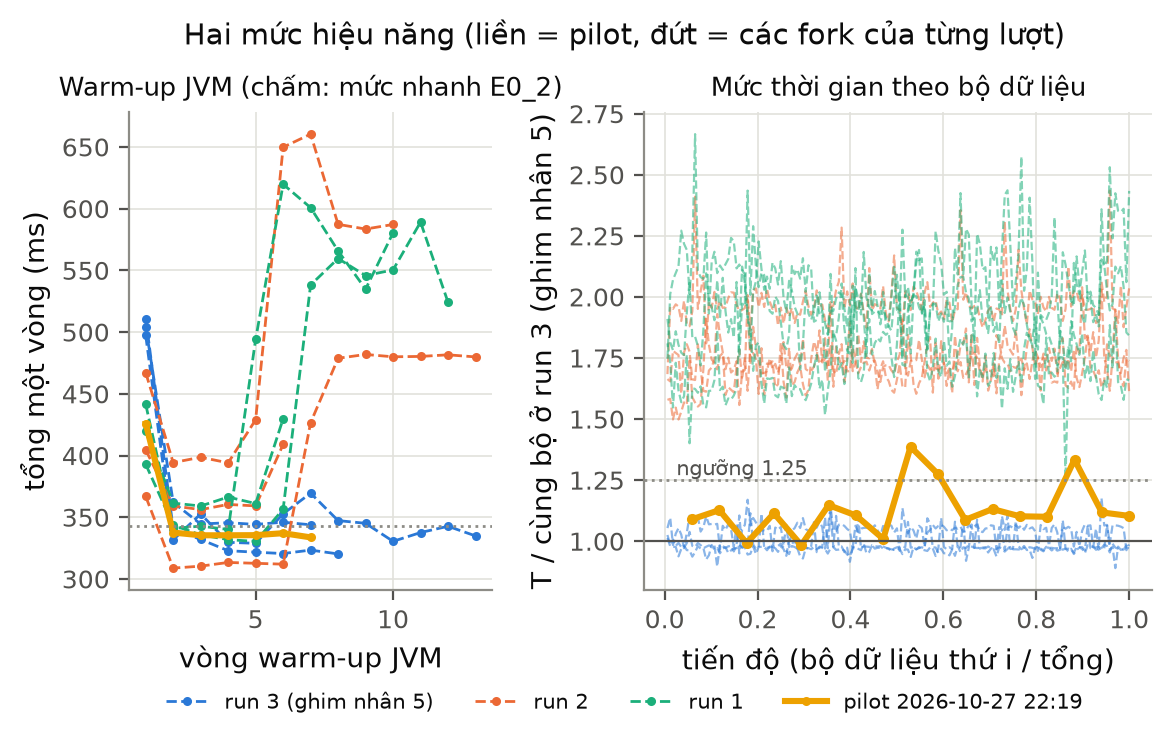
\includegraphics[width=0.95\linewidth]{figures/fig17_jit_state.png}
% Gợi ý chú thích (từ dàn ý): Hai mức hiệu năng ở run 1/2 và các pilot.
\caption{\bv{viết chú thích}}
\label{fig:levels}
\end{figure}

\begin{figure}[H]
\centering
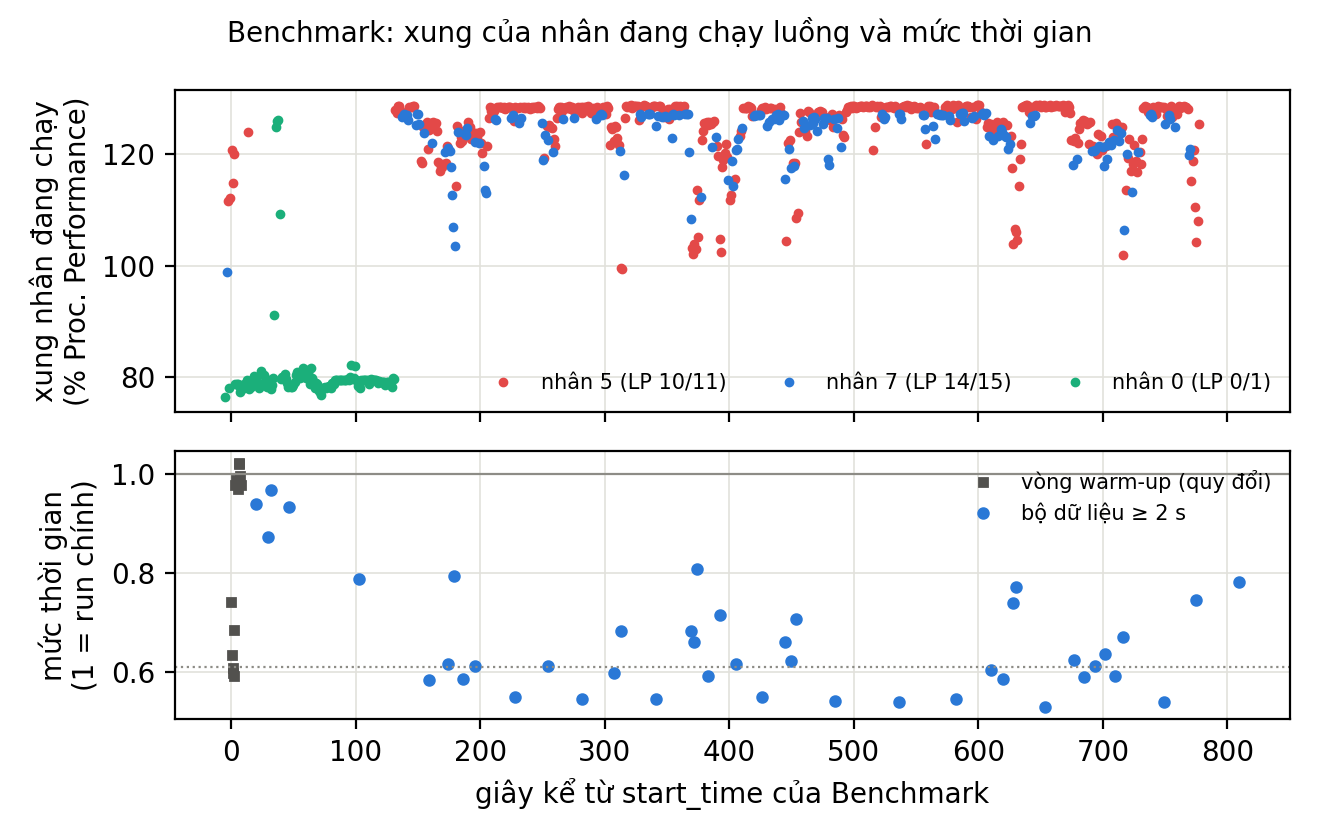
\includegraphics[width=0.95\linewidth]{figures/fig_e6_timeline.png}
% Gợi ý chú thích (từ dàn ý): E6: xung của nhân đang chạy luồng và mức thời gian.
\caption{\bv{viết chú thích}}
\label{fig:e6}
\end{figure}

\begin{figure}[H]
\centering
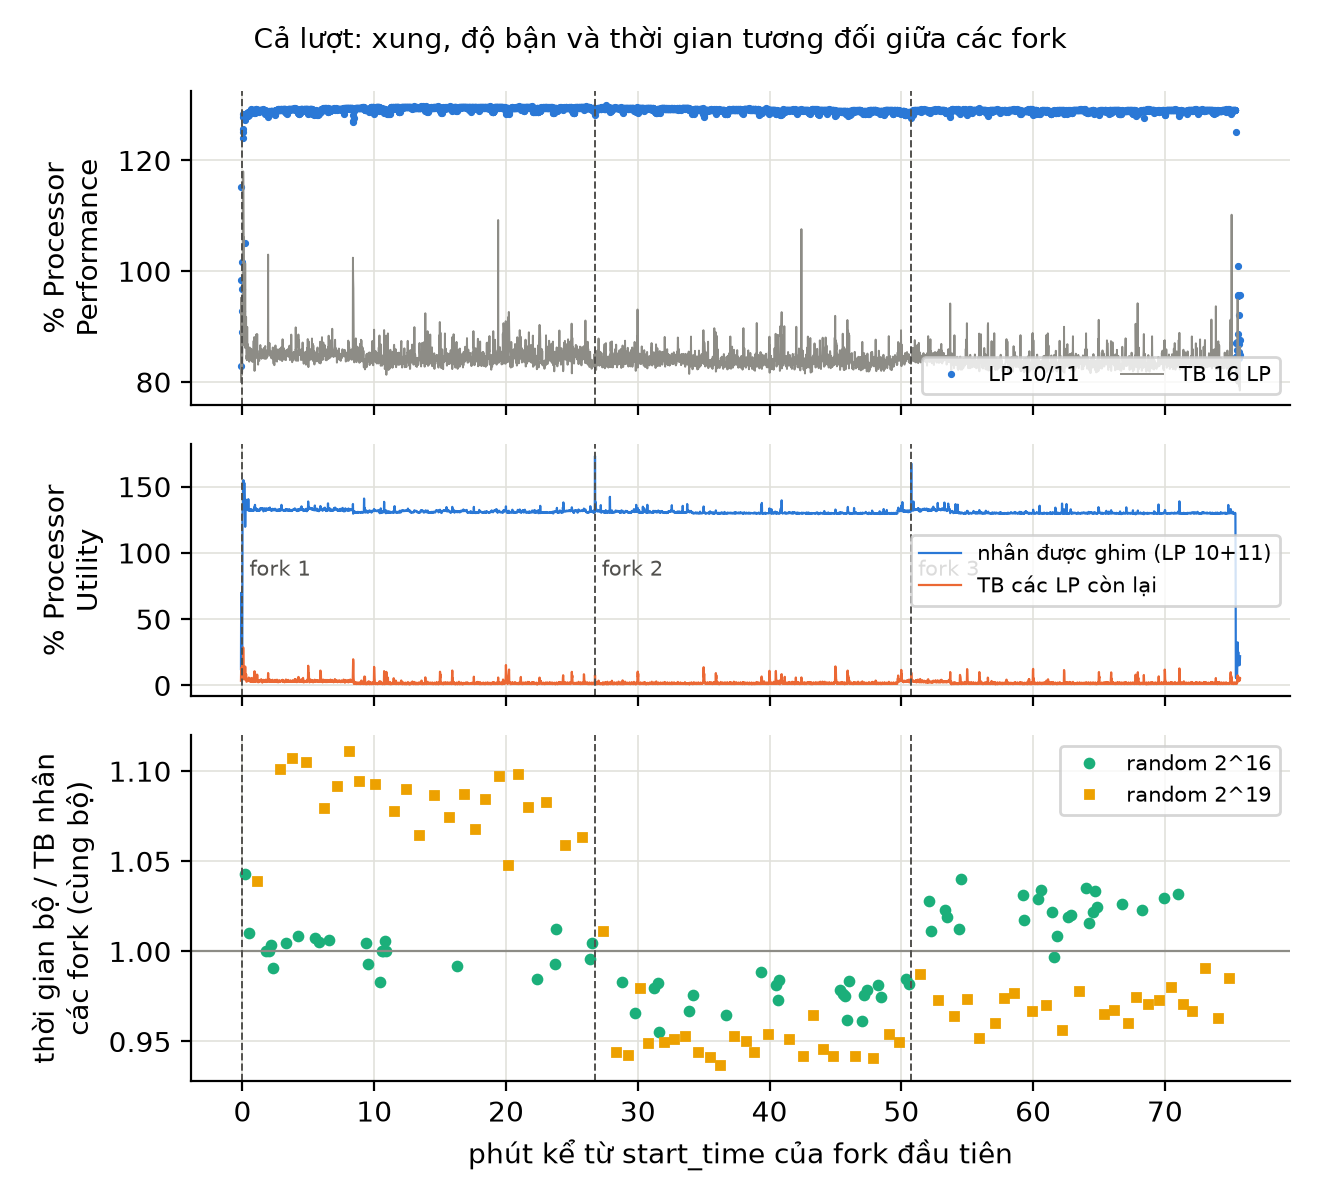
\includegraphics[width=0.95\linewidth]{figures/fig_run3_timeline.png}
% Gợi ý chú thích (từ dàn ý): Run 3: xung, độ bận của nhân được ghim và thời gian tương đối giữa các fork.
\caption{\bv{viết chú thích}}
\label{fig:run3}
\end{figure}


\subsection{Ghim affinity là thay đổi sau khi đã xem dữ liệu}\label{sec:7-2}
%   - Quyết định đưa ra sau run 1/2 và chuỗi chẩn đoán; thiết kế đo khác vẫn giữ nguyên.
%   - Chọn run 3 làm lượt chính cũng là quyết định sau khi đã xem dữ liệu → báo cáo cả 3 lượt (Bảng 6, 7) để người đọc thấy kết luận không phụ thuộc lựa chọn này.
%   - Ghim cả JVM vào một nhân: các luồng phụ của JVM (GC, JIT) dùng chung nhân 5 với luồng đo. Typeperf: nhân 5 bận ~130 (≈ một LP bận hoàn toàn ở xung ~129%). [F78]
%   - Run 3 đại diện cho mức "nhân không phải nhân 0, boost bình thường", không phải trạng thái tự nhiên khi không ghim (khi đó luồng có thể rơi vào nhân 0).
% BẠN VIẾT:
\bv{Bạn viết nội dung phần này}


\subsection{Biến thiên giữa các JVM}\label{sec:7-3}
% (dàn ý) [F64, F79]
%   - CI bootstrap ở bảng 3–4 chỉ lấy mẫu lại theo N, không tính biến thiên giữa các JVM.
%   - Chênh lệch r giữa các fork của run 3 lên tới 2.67% (2^19, c tốt nhất); run 2: 3.69%.
%   - Khoảng t qua 9 JVM:  (S§9).
%   - Run 3 fork 1 chậm hơn fork 2/3 khoảng 8% trên các bộ random 2^19 (24/24 bộ), nhưng không chậm hơn ở 2^16; cùng xung 129.5%, không tương quan với độ bận của các LP khác. Phù hợp với một khác biệt phía bộ nhớ riêng của JVM đó (ví dụ cách cấp phát trang vật lý), chưa kiểm chứng. [F79]
%   - Fork cùng số ở các lượt dùng chung thứ tự bộ dữ liệu, nên không hoàn toàn độc lập.
% - **Run 1 bị nhiễu** do máy mở nhiều ứng dụng và thiếu RAM: SD trong lớp 2.0 / 1.1 / 2.4%, so với 0.7 / 0.4 / 0.4% ở run 3 và 0.8 / 0.5 / 0.4% ở run 2. Kết luận chính không đổi. [F15, F17]
% - **Trôi:** run 3 fork 3 −0.11% mỗi 1 000 lần đo (≈ −3% cả fork; ρ = −0.20). Thứ tự CUTOFF được xáo trong mỗi trial nên r không bị lệch hệ thống. [F12]
% - **Diễn giải về cache chỉ là gián tiếp** [F50–F55]
%   - Run 3: T/(N lgN) tăng +3.8% khi vượt ngưỡng L3 trong thang 2^19; run 2 thì không.
%   - Độ tăng theo N phụ thuộc mức hiệu năng (mục 6), và không đồng nhất giữa các thang.
%   - Các nguyên nhân không tách được: TLB, L3 kiểu victim cache, DRAM single-channel, truy cập Integer qua tham chiếu bị xáo trộn.
% - **Lưới CUTOFF:** tối ưu của đã sắp và gần sắp nằm ở đầu mút 64.
% - **Môi trường:** laptop, không tắt turbo; Windows có tiến trình nền; RAM single-channel; gói nguồn Balanced.
% - **Phạm vi:** chỉ `Integer[]`, chỉ top-down, các cải tiến khác bị tắt. So sánh giữa các phân bố chỉ dựa trên r, vì bố cục bộ nhớ khác nhau.
% - SerialGC có thể di chuyển các đối tượng Integer giữa các lần đo.
%
% BẠN VIẾT:
\bv{Bạn viết nội dung phần này}

\begin{table}[H]
\centering
% Gợi ý chú thích (từ dàn ý): Biến thiên giữa 9 JVM: TB nhân, min–max, khoảng t 95%.
\caption{\bv{viết chú thích}}
\label{tab:perjvm}
\small
\begin{adjustbox}{max width=\linewidth}% Bảng: biến thiên giữa 9 JVM (3 lượt x 3 fork) (T:per_jvm_summary)
% Sinh tự động bởi report/make_tables.py, KHÔNG sửa tay.
\begin{tabular}{llcccc}
\toprule
Thang & Đại lượng & TB nhân & min--max & Khoảng $t$ 95\% & 10 nhanh hơn 7 \\
\midrule
$2^{12}$ & r(7) & 0.8929 & 0.8830--0.9076 & [0.8860, 0.8999] &  \\
 & r(10) & 0.8771 & 0.8680--0.8954 & [0.8705, 0.8836] &  \\
 & r(30) & 0.8214 & 0.8035--0.8355 & [0.8133, 0.8296] &  \\
 & $T_7/T_{10}$ & 1.0181 & 1.0126--1.0247 & [1.0148, 1.0214] & 9/9 \\
\addlinespace
$2^{16}$ & r(7) & 0.9233 & 0.9118--0.9359 & [0.9175, 0.9291] &  \\
 & r(10) & 0.9127 & 0.9007--0.9303 & [0.9056, 0.9197] &  \\
 & r(30) & 0.8814 & 0.8654--0.8941 & [0.8738, 0.8891] &  \\
 & $T_7/T_{10}$ & 1.0116 & 1.0060--1.0151 & [1.0092, 1.0141] & 9/9 \\
\addlinespace
$2^{19}$ & r(7) & 0.9511 & 0.9383--0.9646 & [0.9442, 0.9581] &  \\
 & r(10) & 0.9389 & 0.9282--0.9552 & [0.9324, 0.9455] &  \\
 & r(30) & 0.9208 & 0.9049--0.9467 & [0.9109, 0.9308] &  \\
 & $T_7/T_{10}$ & 1.0130 & 1.0037--1.0306 & [1.0059, 1.0201] & 9/9 \\
\bottomrule
\end{tabular}
\end{adjustbox}
\end{table}


\section{Kết luận}\label{sec:8}
%
% - **RQ1:** trên máy này, mọi CUTOFF trong 22–32, 40, 48 đều nằm trong 2% của tối ưu (random, cả 3 thang, cả 3 lượt). Giá trị tốt nhất khi gộp 3 thang là 30 (run 3); 31 và 40 ở run 2 và run 1. [F25–F27]
% - **RQ2:** mức lợi giảm dần theo N (18.0% → 11.2% → 8.2%). Phân bố dữ liệu làm dịch tối ưu rõ rệt:
%   - đảo ngược ≈ 8–10 (vùng 6–12);
%   - đã sắp / gần sắp ≥ 64.
% - **RQ3:**
%   - Tại 7 và 10, thời gian giảm 5.2–12.6% (run 3); 10 tốt hơn 7 khoảng 0.9–2.1%, ở mọi thang và cả 3 lượt.
%   - Không đạt "20%" theo cách đọc r = 0.80. Chỉ đạt 1.2 lần ở N nhỏ với c tốt nhất (1.219×).
% - **Phương pháp:** kết luận bền qua hai mức xung khác nhau 1.6 lần; thời gian tuyệt đối thì không.
% - **Khuyến nghị gợi ý:** CUTOFF ≈ 24–32 cho dữ liệu chung; nêu kèm điều kiện (máy, JDK, `Integer[]`).
%
% BẠN VIẾT:
\bv{Bạn viết nội dung phần này}


\appendix
%

\section{Tái lập}\label{sec:A}
%   - Cấu trúc thư mục; lệnh `run_all.bat`; lệnh khởi chạy có affinity cho run 3; lệnh `analyze.py` (kèm `--compare` nhiều thư mục, `--compare-label`, `--state-ref`, `--pilots`); lệnh `diag_bench_align.py` cho run 3.
%   - Các giá trị sha256 [F05, F06]; phiên bản Python và JDK; cách tạo lại dữ liệu bằng `DataGenerator --verify`.
% BẠN VIẾT:
\bv{Bạn viết nội dung phần này}

\begin{verbatim}
javac -encoding UTF-8 -d build src\*.java
java -ea -cp build CorrectnessTest
java -cp build DataGenerator --verify
scripts\run_all.bat --high            (run 1, run 2)
:: run 3: ghim nhân 5
cmd /c start "java" /b /wait /high /affinity C00 java -Xms2g -Xmx2g ^
    -XX:+UseSerialGC -XX:+AlwaysPreTouch -cp build Benchmark --fork F --results results_run3
python scripts\analyze.py --results results_run3 --label "run 3 (ghim nhân 5)" ^
    --compare results results_run1 --compare-label "run 2" "run 1"
python report\make_tables.py
\end{verbatim}


\section{Ba lượt chạy}\label{sec:B}
%   - Bảng 6, 7 đầy đủ (mọi phân bố) từ S§11; F:fig15.
%   - Bảng điều kiện từng lượt: ngày giờ, affinity, typeperf có/không, RAM trống từng fork, thời gian thực, mức warm-up so với mức nhanh. [F15, F77, F83]
% BẠN VIẾT:
\bv{Bạn viết nội dung phần này}


\section{Chuỗi chẩn đoán "hai mức hiệu năng"}\label{sec:C}
%   - **Bảng C1** (một dòng mỗi bước; cột: câu hỏi · cách làm · kết quả · kết luận · fact):
%
%     | Bước | Câu hỏi | Cách làm | Kết quả chính | Kết luận | Fact |
%     |---|---|---|---|---|---|
%     | 0 | Có hai mức không? | warm-up JVM, mức theo bộ dữ liệu (S§10) | run 1/2 nhảy ở vòng 5–7, giữ mức chậm; pilot chuyển qua lại | có hai mức, tỉ lệ ~1.6 | F57–F61 |
%     | 1 | Do JIT? | `-XX:+PrintCompilation`, pilot và JVM chính (28/10) | không có sự kiện biên dịch quanh lúc chuyển | loại JIT | F65–F68 |
%     | 2 | Có tái hiện bằng công cụ riêng? | WarmupProbe + typeperf (E0_1, E0_2) | 296/300, 900/900 vòng nhanh; 4 vòng chậm khi luồng sang nhân 0 | gợi ý: nhân 0 | F71, F72 |
%     | 3 | Benchmark chậm ở đâu? | Benchmark như `run_all.bat` + typeperf (E6) | chậm = nhân 0 ở 77–79%; nhanh = nhân 5/7 ở 125–128% | cơ chế trực tiếp: xung của nhân 0 | F74–F76 |
%     | 4 | Nhân 0 bị giới hạn phần cứng? | ghim nhân 0 / nhân 5 (T2) | nhân 0 lên 123.6–127% khi bị ghim; gói nguồn min 80% | không; mức 79% ≈ mức sàn của gói nguồn | F81, F82 |
%     | 5 | Ghim nhân 5 có giữ mức nhanh cả lượt? | run 3 + typeperf | 100% mẫu trên nhân 5, 128–129.5%; không bước nhảy | có | F77, F78, F83 |
%     | 6 | §10 cũ báo "chậm" trong run 3? | ghép typeperf + so chéo fork (D3) | không có tụt xung; f1 +8% chỉ ở 2^19; f3 dao động quanh ngưỡng | ngưỡng cũ không phù hợp; đổi §10 theo run 3 | F79, F80 |
%
%   - Hình: F:fig17 (hai mức hiệu năng), `diag/E6/bench_timeline.png` (E6), `D3/run_timeline.png` (run 3: xung, độ bận, thời gian tương đối giữa các fork).
%   - Hình chẩn đoán khác: F:fig11 (warm-up), F:fig12 (trôi), F:fig13 (forks), F:fig04 (ghép cặp từng N).
% BẠN VIẾT:
\bv{Bạn viết nội dung phần này}

\begin{table}[H]
\centering
% Gợi ý chú thích (từ dàn ý): Chuỗi chẩn đoán hai mức hiệu năng.
\caption{\bv{viết chú thích}}
\label{tab:diag}
\small
\begin{adjustbox}{max width=\linewidth}% Bảng: chuỗi chẩn đoán hai mức hiệu năng (số liệu từ diag/ và results_run3/diag)
% Sinh tự động bởi report/make_tables.py, KHÔNG sửa tay.
\begin{tabular}{lp{0.33\linewidth}p{0.42\linewidth}}
\toprule
Bước & Cách làm & Kết quả đo \\
\midrule
PrintCompilation & 2 JVM, \texttt{-XX:+PrintCompilation} & không có sự kiện biên dịch MergeCutoff quanh lúc chuyển mức \\
Pilot A/B & pilot sau 10 phút nghỉ; pilot chạy liền sau & cả hai không nhảy ở warm-up \\
E0\_1, E0\_2 & WarmupProbe 300 / 900 vòng + typeperf & 296/300 và 900/900 vòng nhanh; xung $\approx$121\% \\
E6 & Benchmark như \texttt{run\_all.bat} + typeperf & 3.4--130.9 s trên nhân 0 ở 77--79\%; sau đó nhân 5/7 ở 125--128\% \\
T2\_c0 & ghim nhân 0 (\texttt{/affinity 3}) & nhân 0 ở 124--127\%, nhanh \\
T2\_c5 & ghim nhân 5 (\texttt{/affinity C00}) & nhân 5 ở $\approx$128\%, nhanh \\
run 3 & 3 fork, ghim nhân 5 + typeperf suốt lượt & 100\% mẫu trên nhân 5; xung trung vị 129.0--129.5\% \\
\bottomrule
\end{tabular}
\end{adjustbox}
\end{table}

\begin{figure}[H]
\centering
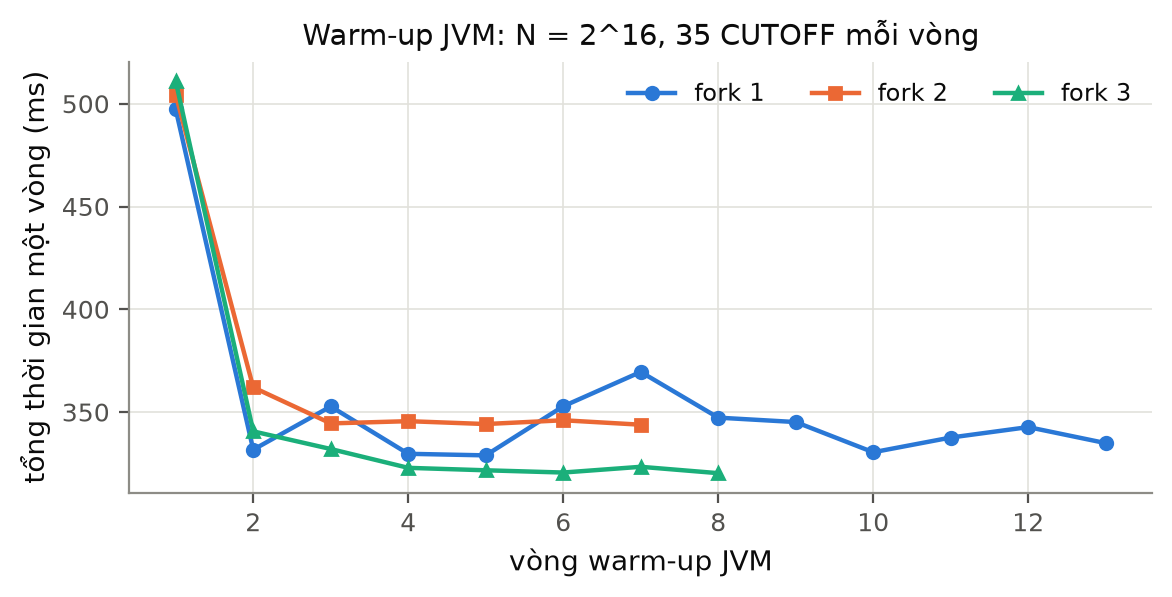
\includegraphics[width=0.8\linewidth]{figures/fig11_jvm_warmup.png}
% Gợi ý chú thích (từ dàn ý): Warm-up JVM.
\caption{\bv{viết chú thích}}
\label{fig:warmup}
\end{figure}

\begin{figure}[H]
\centering
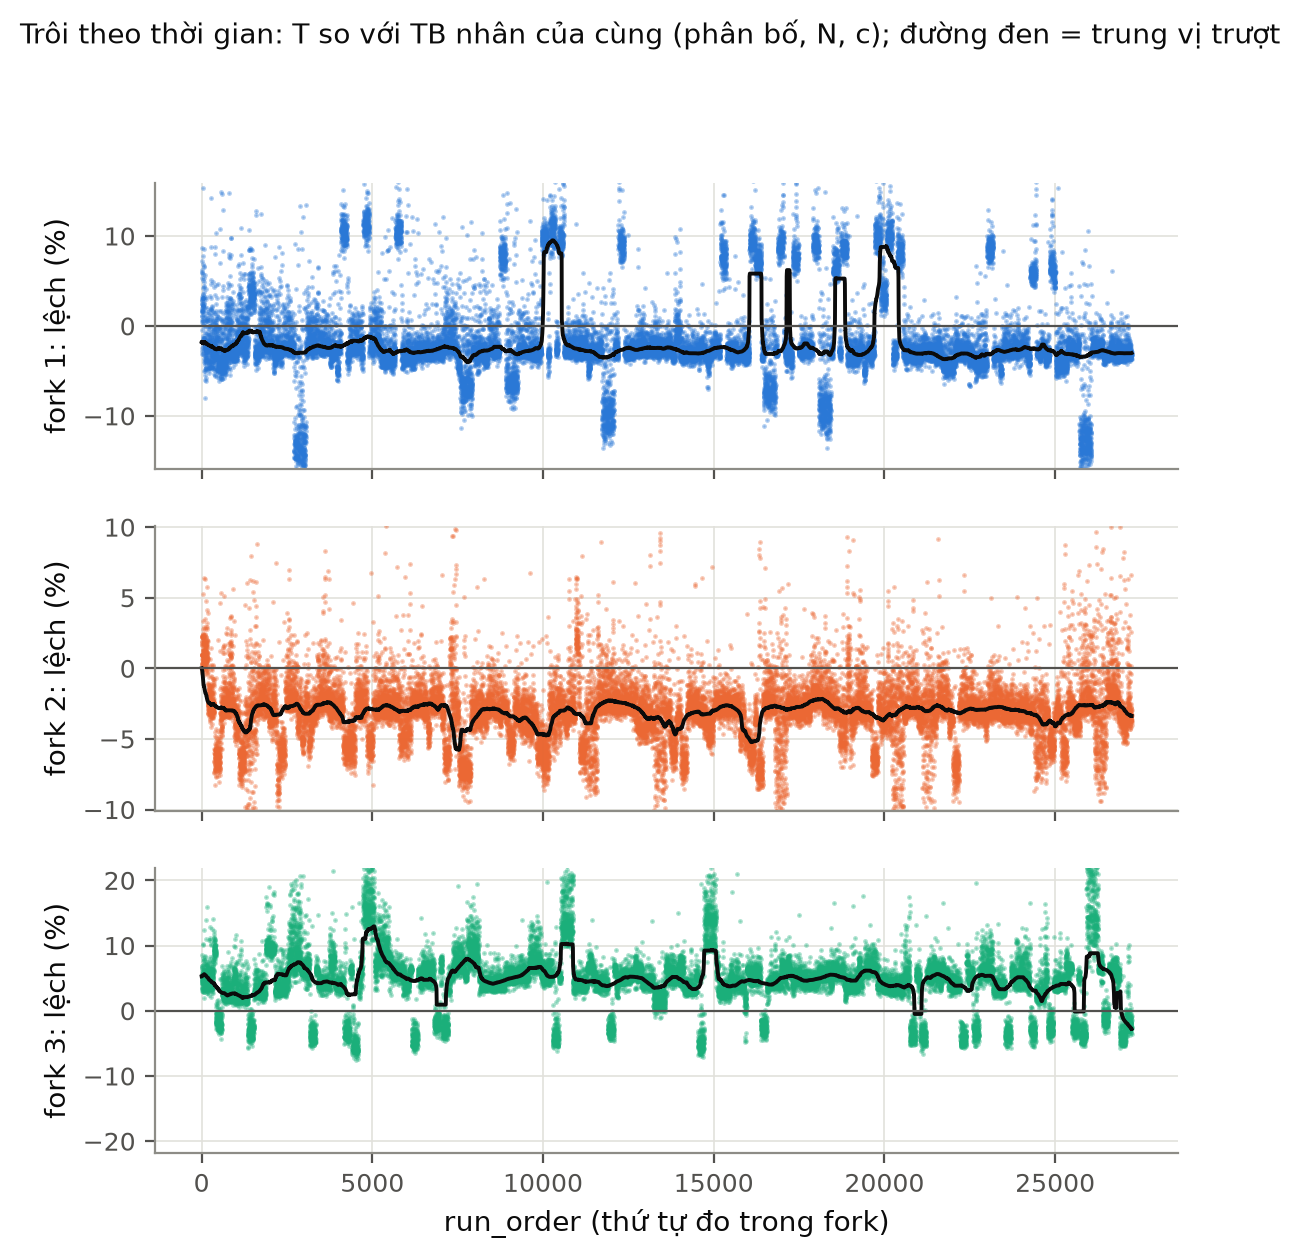
\includegraphics[width=0.8\linewidth]{figures/fig12_drift.png}
% Gợi ý chú thích (từ dàn ý): Trôi theo thứ tự đo.
\caption{\bv{viết chú thích}}
\label{fig:drift}
\end{figure}

\begin{figure}[H]
\centering
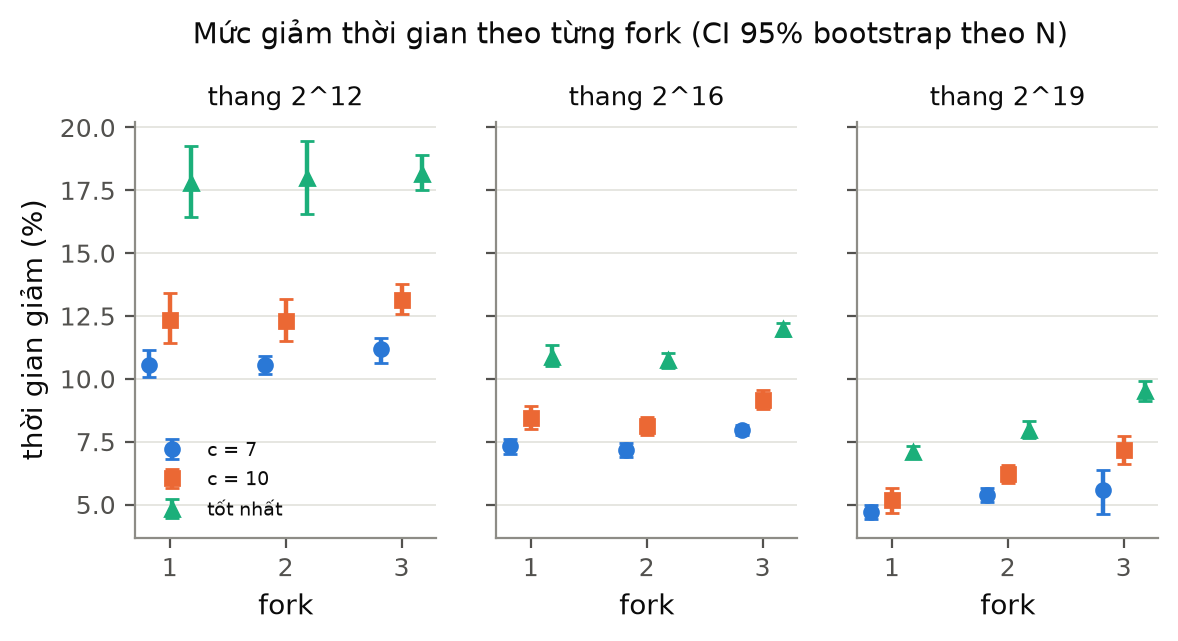
\includegraphics[width=0.8\linewidth]{figures/fig13_forks.png}
% Gợi ý chú thích (từ dàn ý): So sánh giữa các fork.
\caption{\bv{viết chú thích}}
\label{fig:forks}
\end{figure}

\begin{figure}[H]
\centering
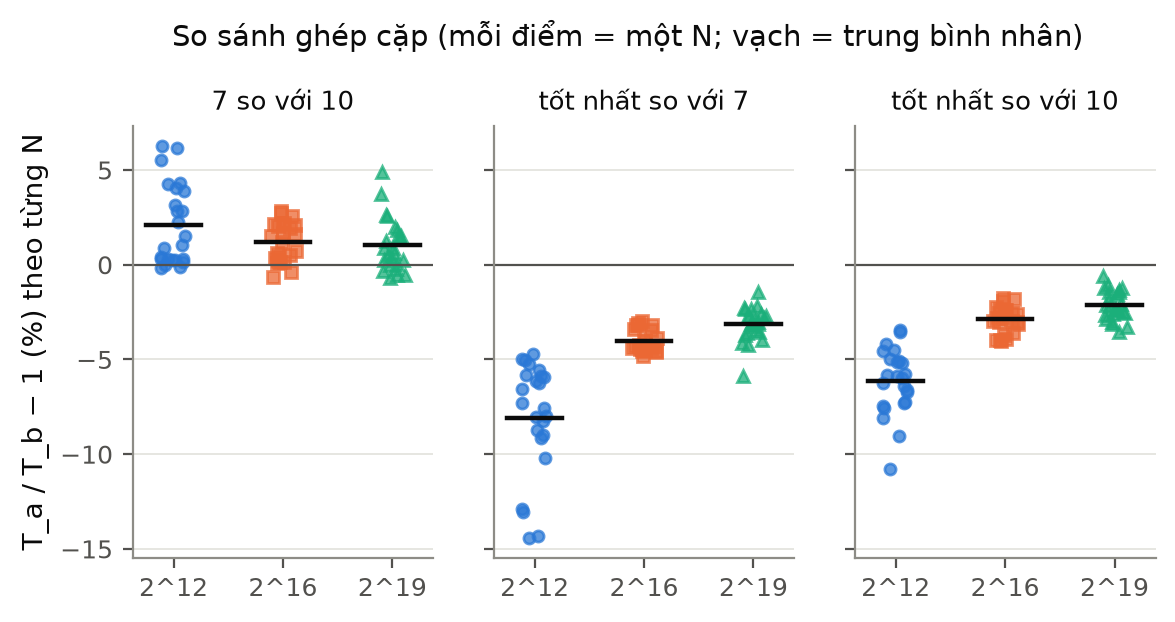
\includegraphics[width=0.8\linewidth]{figures/fig04_paired_differences.png}
% Gợi ý chú thích (từ dàn ý): Chênh lệch ghép cặp theo từng N.
\caption{\bv{viết chú thích}}
\label{fig:paired}
\end{figure}


\section{Tuyên bố sử dụng AI}\label{sec:D}
% (dàn ý) (bạn tự viết; các ý cần có cho đúng sự thật):
%   - **AI đã làm:**
%     - Thảo luận và review thiết kế thí nghiệm.
%     - Review `MergeCutoff.java`: chỉ ra lỗi, không viết lại.
%     - Viết `MergeCutoffCounted.java` bằng cách chèn bộ đếm vào code của bạn.
%     - Viết `CorrectnessTest`, `DataGenerator`, `Benchmark`, `CountRunner`, các file `.bat`, `analyze.py`, và các công cụ chẩn đoán (`WarmupProbe`, `diag_probe.ps1`, `diag_align.py`, `diag_bench_align.py`).
%     - Đo kích thước đối tượng và chạy mutation test trên sandbox.
%     - Phân tích log PrintCompilation và typeperf; đề xuất các thí nghiệm chẩn đoán.
%   - **Bạn đã làm:** cài đặt `MergeCutoff.java`, mọi lần chạy đo và chẩn đoán trên máy bạn, quyết định ghim nhân và chọn lượt chính, và toàn bộ văn bản báo cáo.
%   - Log đầy đủ: `ai_log/`.
%
% ---
%
% BẠN VIẾT:
\bv{Bạn viết nội dung phần này}


\nocite{*}
\bibliographystyle{plain}
\bibliography{refs}
\end{document}
